\documentclass[review,12pt]{elsarticle}

\usepackage{amsmath, amssymb}
\usepackage{graphicx}
\usepackage{float}
\usepackage{adjustbox}
\usepackage{multirow}
\usepackage{array}
\usepackage{makecell}
\usepackage{tabularx}
\usepackage{textcomp}
\usepackage{longtable}
\usepackage{microtype}
\newcommand{\degree}{\ensuremath{^\circ}}
\usepackage{lineno}
\usepackage[hyphens]{url}
\usepackage{hyperref}
\pdfstringdefDisableCommands{%
  \def\corref#1{}%
  \let\cnotenum\relax
  \let\@corref\relax
}

\modulolinenumbers[5]

\bibliographystyle{elsarticle-harv}

\journal{International Communications in Heat and Mass Transfer}
\makeatletter
\def\ps@pprintTitle{%
  \let\@oddhead\@empty
  \let\@evenhead\@empty
  \def\@oddfoot{\scriptsize\itshape Preprint submitted to \ifx\@journal\@empty Elsevier\else\@journal\fi\hfill\today}%
  \let\@evenfoot\@oddfoot}
\makeatother

\begin{document}

\begin{frontmatter}

\title{Parametric Thermo-Hydraulic Benchmarking of Capsule and Dimple Plate Heat Exchanger Channels via Periodic Unit-Cell CFD}

\author[rmit]{Cheuk Sing Cheung}
\author[rmit]{Christos Skarakis}
\author[inkorr]{Lance Smith}
\author[rmit]{Sara Vahaji\corref{cor1}}
\cortext[cor1]{Corresponding author}
\ead{sara.vahaji2@rmit.edu.au}

\address[rmit]{School of Engineering, RMIT University, Melbourne, VIC 3000, Australia}

\address[inkorr]{InKorr Pty Ltd, Knoxfield, VIC 3180, Australia}

\begin{abstract}
Plate heat exchangers increasingly use non-chevron embossing (e.g., capsule and dimple patterns) to improve thermal performance while limiting pressure penalties, yet designers lack consistent, head-to-head guidance on how core geometric parameters control the thermal--hydraulic trade-off across these pattern families. This study presents a unified unit-cell CFD benchmarking of capsule-type and dimple-type plate heat exchanger channels under a consistent hydraulic-diameter definition and identical boundary conditions. Capsule angle and height, and dimple height and spacing, are systematically varied over manufacturing-relevant ranges, and their impacts on friction factor, pressure drop, and Nusselt number are interpreted through turbulence kinetic energy, streamline topology, and temperature-field evolution. A Relative Embossing Depth (RED\,=\,$h/D_e$) is introduced to map all 27 parametric cases onto a single dimensionless geometric axis, and a Thermal Performance Factor (TPF\,=\,Nu/$f^{1/3}$) is used to rank every case on an identical thermo-hydraulic scale. The cross-family comparison reveals that dimple-type plates consistently outperform capsule-type plates in TPF, with tall dimples ($D_h$\,$\geq$\,4.0\,mm) and closely spaced dimples ($D_s$\,$\leq$\,3.2\,mm) occupying the top of the ranking, while capsule-angle cases cluster in the lower half. The framework, performance metrics, and resulting design-selection rules provide actionable guidance for choosing and tuning capsule versus dimple embossing in next-generation compact PHEs, including high-density data-center liquid-cooling applications.
\end{abstract}

\begin{keyword}
CFD \sep Plate heat exchangers \sep Capsule-type PHE \sep Dimple-type PHE \sep Heat transfer \sep Thermal performance factor
\end{keyword}

\end{frontmatter}

\linenumbers

\begin{table}[H]
\caption{Nomenclature}
\centering
\scriptsize
\renewcommand{\arraystretch}{1.05}
\begin{tabular}{@{}ll@{\quad}ll@{}}
\hline
\textbf{Symbol} & \textbf{Description} & \textbf{Symbol} & \textbf{Description} \\
\hline
$A_0$       & Inlet area (mm$^2$) & Nu          & Nusselt number (--) \\
$C_h$       & Capsule height (mm) & Pr          & Prandtl number (--) \\
$C_p$       & Specific heat capacity (J/kg$\cdot$K) & $\Delta p$  & Pressure drop (Pa) \\
$D$         & Dimple diameter (mm) & Re          & Reynolds number (--) \\
$D_e$       & Hydraulic diameter (mm) & RED         & Relative Embossing Depth (--) \\
$D_h$       & Dimple height (mm) & $S$         & Total heat transfer area (mm$^2$) \\
$D_s$       & Dimple edge-to-edge gap (mm) & TPF         & Thermal Performance Factor (--) \\
$f$         & Fanning friction factor (--) & $u$         & Inlet velocity (m/s) \\
$h$         & Embossing height (mm) & $w$         & Capsule width (mm) \\
$h_{ave}$   & Avg.\ heat transfer coeff.\ (W/m$^2\cdot$K) & $y^+$       & Dimensionless wall distance (--) \\
$l$         & Capsule length (mm) & ~ & ~ \\
$l_c$       & Unit cell length (mm) & ~ & ~ \\
$l_d$       & Dimple unit cell length (=$l_c$) (mm) & ~ & ~ \\
$p$         & Dimple pitch (mm) & ~ & ~ \\
\hline
\multicolumn{2}{l}{\textbf{Greek symbols}} & \multicolumn{2}{l}{\textbf{Abbreviations}} \\
\hline
$\delta$    & Boundary layer thickness (m) & CFD   & Computational Fluid Dynamics \\
$\theta_c$  & Capsule angle (\degree) & CPHE  & Capsule-Type PHE \\
$\lambda$   & Thermal conductivity (W/m$\cdot$K) & DPHE  & Dimple-Type PHE \\
$\rho$      & Fluid density (kg/m$^3$) & PHE   & Plate Heat Exchanger \\
$\upsilon$  & Kinematic viscosity (m$^2$/s) & RANS  & Reynolds-Averaged Navier--Stokes \\
            &                               & SST   & Shear Stress Transport \\
            &                               & STHE  & Shell and Tube Heat Exchanger \\
            &                               & TKE   & Turbulence Kinetic Energy \\
\hline
\end{tabular}
\end{table}

\clearpage

\section{Introduction}
\label{sec:introduction}


In the pursuit of sustainable engineering and energy efficiency, advancing heat exchanger designs has become critically important. Heat exchangers are vital in various industries, including power generation, chemical processing, HVAC, and the rapidly expanding data-center sector---where liquid cooling of high-density server racks used to train and deploy artificial intelligence models demands compact, high-performance thermal solutions---and their performance directly impacts operational costs and energy consumption. 

Among heat exchanger types, Shell and Tube Heat Exchangers (STHEs) and Plate Heat Exchangers (PHEs) are commonly used. STHEs are valued for their robustness and capacity to handle high pressures. Recent innovations such as helical baffles have enhanced mixing and heat transfer while reducing pressure drops and dead zones \citep{salahuddin2015}. However, STHEs face challenges in manufacturing complexity and design benchmarking.

Conversely, PHEs are gaining popularity in industries such as manufacturing, air conditioning, and refrigeration due to their compactness, ease of cleaning, and adaptability. Composed of stacked metallic plates, PHEs offer higher thermal efficiency and a larger surface area per volume compared to STHEs \citep{abukhader2012}. They can reduce spatial requirements by up to 40\% on the cold side and 25\% on the hot side, operating efficiently between 10--20 bar. Their design also supports higher wall shear, reducing fouling rates. PHEs typically experience fouling factors around 20--25\% of those seen in STHEs \citep{thulukkanam2013}.

Despite their benefits, PHEs have limitations, notably pressure (up to 20.4 bar) and temperature caps (around 150\degree C). Specialized designs, such as brazed or welded PHEs, can extend operational limits. However, high turbulence needed for performance also induces higher pressure drops. Ongoing research is focused on reducing pressure loss while maintaining thermal efficiency.

The plate configuration is central to a PHE's performance. The chevron (or herringbone) pattern is widely used and extensively studied, with research focusing on chevron angles, channel depth, and stacking arrangements. More than 60 alternative plate patterns have been introduced, some surpassing the chevron in performance. Passive surface enhancement strategies---like embossed, roughened, or corrugated plates---are gaining traction \citep{zhang2019a}.

Embossed surfaces, such as capsule, dimple, and pillow types, have been shown to reduce fouling and pressure losses while improving maintenance and thermal performance. \citet{hamedi2024} found that symmetrical convex/concave capsule arrangements improved friction factors by 35--44\% and the Nusselt number by 28--55\%. \citet{jiang2019a} demonstrated that capsule length-to-width ratios impact heat exchanger performance; larger ratios enhance energy efficiency, while smaller ratios improve heat transfer at the cost of pressure loss. These studies have shown that symmetrical capsule arrangements outperform traditional zig-zag patterns. Smaller capsules promote heat transfer, whereas larger ones minimize pressure losses.

Capsule embossing has also demonstrated superior Nusselt numbers and lower friction factors compared to chevron patterns. Optimization methods using CFD and multi-objective algorithms have improved heat transfer coefficients while reducing friction coefficients \citep{yu2024}.

Hybrid enhancements---like adding dimples to capsules or pillow-type surfaces can further increase performance. \citet{shao2024} found that combining dimples with capsule surfaces enhanced heat transfer by 19--46\%. Similarly, dimpled pillow plates improved thermo-hydraulic performance by 11.2\% and reduced pressure loss by 8.7\% \citep{piper2019}. While advancements are notable, further research is needed to explore novel embossing patterns and benchmark existing configurations. For example, previous studies have explored the potential of combining secondary structures, such as dimples, with capsule or pillow-type surfaces, demonstrating promising performance gains. While this hybrid approach remains underexplored, it highlights the broader need for deeper investigation into how arrangement patterns---whether in standalone capsule or dimple configurations---can enhance flow mixing and thermal performance. This study contributes to that effort by focusing specifically on standalone capsule and dimple designs.

This study addresses the current research gaps in understanding how individual geometric features influence thermo-hydraulic performance in non-chevron PHE designs. Specifically, it conducts a numerical investigation of capsule- and dimple-type plate heat exchangers (PHEs), focusing on how variations in capsule angle and height, as well as dimple height and spacing, affect flow behavior, pressure drop, and heat transfer efficiency. The goal is to provide practical design guidelines for next-generation heat exchangers. Earlier work by \citet{jiang2019} highlighted the influence of capsule length-to-width ratios on heat transfer and pressure loss. Symmetrical capsule arrangements outperformed zig-zag configurations, and dimensions influenced performance depending on application needs. \citet{hamedi2024} confirmed that symmetrical convex/concave capsule patterns reduced friction and improved Nusselt numbers. Further, aligned embossing directions (e.g., convex on convex) performed better than alternating arrangements.

\citet{yu2024} introduced a CFD-based optimization approach using a backpropagation algorithm to adjust parameters such as capsule angle and length. Their method improved heat transfer coefficients by 8.3\% while reducing friction by 14.3\%. Studies on pillow-type embossing also highlight benefits. \citet{shirzad2019a} optimized internal channel height and welding spot distances, achieving peak efficiency at a 36 mm longitudinal distance and increased transversal spacing. \citet{arsenyeva2019} found pillow plates required 30\% less heat transfer area than chevron types, reducing pressure drops.

\citet{shao2024} explored secondary dimples in capsule-type designs, achieving heat transfer improvements of 19--46\%, albeit with increased flow resistance. \citet{piper2019} reported a 2.2\% rise in heat transfer and an 8.7\% drop in pressure loss for dimpled pillow designs. Table~\ref{tab:embossing-summary} summarizes the investigations on embossing surface enhancements for PHEs. PHEs continue to be a central focus due to their versatility. Experimental and numerical analyses across multiple fluid types show consistent findings. \citet{mocnik2020, mocnik2023, mocnik2024} compared turbulent models and validated numerical accuracy for single-phase water flows using the $k$--$\epsilon$ realizable model, demonstrating better agreement than $k$--$\omega$ SST models.

Expanding on prior studies, this study evaluates the influence of specific geometric modifications on pressure drop, friction factor, and heat transfer. While previous investigations on surface enhancements for PHEs have largely focused on individual embossing families independently, a direct comparative analysis has remained elusive due to inconsistent modeling assumptions across the literature. The presented study addresses this gap by establishing a unified CFD benchmarking framework for capsule-type and dimple-type non-chevron plate geometries. By employing a consistent periodic unit-cell domain and a common hydraulic-diameter definition for periodically varying channels, we ensure an ``apples-to-apples'' comparison of the said patterns. We quantify four manufacturing-relevant geometric parameters (capsule angle and height; dimple height and spacing) and the numerical results indicate these parameters do not merely scale performance but fundamentally shift the thermal--hydraulic trade-off. The results are also synthesized into design-selection regimes based on the objective function of the system (energy-constrained: minimize $f$; heat-demanding: maximize Nu; and balanced operation: best Nu/$f^{1/3}$) and identify three primary mechanisms governing the heat-transfer enhancements: wake interaction, recirculation, and turbulence redistribution. Consequently, these findings yield a robust set of design selection guidelines that facilitate the strategic selection between capsule and dimple embossing, aligning the surface architecture with the specific thermo-hydraulic requirements for next-generation compact PHEs.

\footnotesize
\setlength{\LTleft}{0pt}
\setlength{\LTright}{0pt}
\begin{longtable}{@{\extracolsep{\fill}}>{\raggedright}p{2.6cm} >{\raggedright}p{1.6cm} >{\raggedright}p{1.6cm} >{\raggedright\arraybackslash}p{7cm}@{}}
\caption{Summary of embossing surface enhancement of PHEs.}
\label{tab:embossing-summary} \\
\hline
\textbf{Author} & \textbf{Surface} & \textbf{Method\textsuperscript{a}} & \textbf{Key Findings} \\
\hline
\endfirsthead
\caption[]{(continued)} \\
\hline
\textbf{Author} & \textbf{Surface} & \textbf{Method\textsuperscript{a}} & \textbf{Key Findings} \\
\hline
\endhead
\hline
\endfoot
\citet{hamedi2024} & Capsule & E \& N & Proposed a new symmetrical pattern arrangement for convex/concave capsule surfaces. Friction factor improved by 35--44\%; Nusselt number increased by 28--55\%. \\
\citet{jiang2019a} & Capsule & N & Investigated the effect of capsule length-to-width ratio on performance. A larger ratio improves energy efficiency; a smaller ratio increases heat transfer but raises pressure drop. \\
\citet{jiang2020} & Capsule & N & Symmetrical pattern of capsule allocation performs better than zig-zag. Smaller capsule sizes are better for high heat transfer; larger sizes reduce pressure loss. \\
\citet{jiang2019} & Capsule & E & Experimental studies on flow behaviors have indicated that the geometry of plate corrugation has minimal impact on the distribution of liquid and gas in plate channels during two-phase flow. \\
\citet{zhang2016} & Capsule & E \& N & Capsule embossing shows a higher Nusselt number and lower friction factor compared to chevron-type surfaces. \\
\citet{yu2024} & Capsule & N & Optimization via CFD + backpropagation algorithm. Improved heat transfer coefficient by 8.3\%, friction reduced by 14.3\%. \\
\citet{shao2024} & Capsule / Dimple & N & Secondary dimples added to capsule surfaces. Heat transfer enhanced by 19--46\%. \\
\citet{arsenyeva2019} & Pillow & E \& N & 30\% lower heat transfer area required than chevron type, less pressure drop can be obtained. \\
\citet{shirzad2019a} & Pillow & N & The findings suggest that a greater internal height at low Reynolds numbers and increased transversal distance of welding spots at high Reynolds numbers offer the highest efficiency. \\
\citet{shirzad2019b} & Pillow & N & Numerical study shows that nanofluid as the fluid medium of heat transfer shows better thermal performance than water. \\
\citet{kumar2019} & Pillow & N & Heat transfer and fluid flow characteristics of the pillow plate channel have been numerically studied. \\
\citet{piper2019} & Pillow / Dimple & N & Thermo-hydraulic performance improved by 11.2\%; pressure loss reduced by 8.7\%. \\
\citet{jing2019} & Dimple & N & Numerical study of Supercritical CO$_2$ flow and heat transfer in rectangular channels with teardrop dimple. \\
\citet{li2019} & Dimple & E & Experimental studies on two-phase flow indicated that smaller air bubbles exhibit superior heat transfer performance compared to medium and large bubbles. \\
\citet{mocnik2020} & Dimple & E \& N & Comparison of different turbulent models in numerical study and experimental results, two flow regimes were identified. \\
\citet{mocnik2023} & Dimple & E \& N & Simulation results were in the band between $-$11\% to 1.8\% comparing to experimental result. \\
\citet{mocnik2024} & Dimple & E \& N & Numerical results show good correlation to the experimental results for low Reynolds number flow in Dimple type PHE. \\
\citet{soman2019} & Dimple & E & Dimple-type PHE provides improved heat transfer when using nanofluids compared to water, without a concurrent increase in the friction factor. \\
\citet{soman2022} & Dimple & N & Compared dimple PHE to flat PHE. Nusselt number improved by 39\%. \\
\citet{torre2019} & Dimple & E \& N & A satisfactory consensus was observed regarding pressure drop and heat transfer of PHE with lubricant and oil as fluid medium. \\
\citet{wang2019} & Dimple & N & Results show that a 20.57\% reduce in pressure drop and 173.6\% increase in net power generated for dimpled surface. \\
\citet{ying2021} & Dimple & E \& N & Heat transfer performance results show that the heat transfer coefficient of hemispherical dimple channels is about 27.2\% higher than rhombus dimple channels. \\
\hline
\multicolumn{4}{l}{\textsuperscript{a}E -- Experimental; N -- Numerical.}
\end{longtable}

\section{Methodology}
\label{sec:methodology}

This numerical investigation employs a computational fluid dynamics (CFD) framework to quantify and benchmark the thermo-hydraulic performance of CPHE and DPHE. Drawing on established literature \citep{jiang2019, mocnik2020}, the methodology integrates periodic unit cell reduction, mesh independence studies, validated turbulence modeling, and comprehensive parametric analysis. 

\subsection{Numerical methods}
\label{sec:numerical_methods}

Reynolds Averaged Navier--Stokes Simulation (RANS) approach is widely adopted in numerical studies of CPHE and DPHE. For example, the turbulence model Realizable $k$--$\epsilon$ was used by \citet{kumar2019, jing2019, mocnik2020, mocnik2024}, where SST $k$--$\omega$ was used by \citet{hamedi2024, jiang2019a, jiang2020, mocnik2020, mocnik2024, torre2019}. In addition, Reynolds stress model \citep{shao2024, mocnik2023}, Elliptic blending $k$--$\epsilon$ \citep{arsenyeva2019, piper2019} and standard $k$--$\epsilon$ \citep{soman2022} are some other widely adopted turbulence models. In this study, the turbulent model SST $k$--$\omega$ is adopted due to its advantages on predicting the near wall behavior, through combining the features of $k$--$\omega$ and $k$--$\epsilon$, it also performs well in areas where flow separation and adverse pressure gradients occurs \citep{kanaris2006, khail2023, menter1994}, which is capable to predict the flow parameters of the complex geometry of this study. 

This study focuses on the heat transfer performance of CPHE and DPHE under sub-critical pressure and temperature conditions of water; thus, a single-phase water flow is adopted for the study. In addition, a steady state condition is set for all simulations.

Due to the complexity of the geometry of CPHE and DPHE, the local hydraulic diameter varies periodically; the hydraulic diameter calculation suggested by \citet{jiang2019a, zohuri2017} will be adopted to determine the hydraulic diameter $D_e$ of the channel:
\begin{equation}
D_e=\frac{4A_0 l_c}{S}
\label{eq:De}
\end{equation}
where $A_0$ is the inlet area, $l_c$ is the unit-cell length, and $S$ is the total heat transfer area on one fluid side of PHE. For all CPHE cases and for the DPHE dimple-height cases, $l_c = l_d = 22.4$~mm. For the DPHE dimple-spacing cases, because the unit cell must accommodate two dimples plus their gaps, $l_c$ changes with $D_s$ according to $l_c = l_d = 2(D + D_s)$. The defined $D_e$ applies to the flow area, which is expanding and contracting across flow cross-sections along the flow length. The concept of a unit cell will be discussed in the geometry section. Reynolds number Re is defined as follows:
\begin{equation}
\text{Re}=\frac{uD_e}{\upsilon}
\label{eq:Re}
\end{equation}
where $u$ and $\upsilon$ indicate the inlet velocity and kinematic viscosity of the fluid, respectively. Fanning friction factor ($f$) is adopted for this study and is defined as follows:
\begin{equation}
f=\frac{\Delta p \, D_e}{2\rho \, l_c \, u^2}
\label{eq:f}
\end{equation}
where $\rho$ is fluid density, and $\Delta p$ is the pressure drop from inlet to outlet. Nusselt number Nu and molecular Prandtl number Pr are defined as follows:
\begin{equation}
\text{Nu}=\frac{h_{ave} D_e}{\lambda} 
\label{eq:Nu}
\end{equation}
\begin{equation}
\text{Pr}=\frac{\upsilon\rho C_p}{\lambda}
\label{eq:Pr}
\end{equation}
where $h_{ave}$, $C_p$, and $\lambda$ represent the average heat transfer coefficient of the plates, specific heat capacity of the fluid, and the thermal conductivity of the fluid, respectively.

In this study, the fluid properties ($\lambda$, $\rho$, $\upsilon$, $C_p$) remain constant as follows: $\lambda = 0.6$~W/m$\cdot$K, $\rho = 998.2$~kg/m$^3$, $\upsilon = 1.00481 \times 10^{-6}$~m$^2$/s, and $C_p = 4182$~J/kg$\cdot$K. The initial Reynolds number is held constant across all investigated geometry cases (see Table~\ref{tab:geom_cases}) to ensure dynamic similarity at the start of each parametric simulation. Re may vary during the iterative process used to reach fully developed flow conditions (see Section~\ref{sec:periodic_boundary}), thereby isolating the effects of geometric variations on the resulting turbulent statistics.

\subsection{Geometry}
\label{sec:geometry}

Two distinct geometrical configurations of plate heat exchangers are considered in this study: the Capsule-Type Plate Heat Exchanger (CPHE) and the Dimple-Type Plate Heat Exchanger (DPHE). Both configurations are designed to intensify heat transfer by inducing complex three-dimensional flow structures through surface embossing, but each uses different geometric patterns---capsule-shaped and dimple-shaped features, respectively.

To maintain high computational efficiency without compromising the fidelity of simulation results, a unit cell reduction strategy is employed. By leveraging the periodic nature of the heat exchangers' surface features, a representative segment of the full plate---the unit cell---is modelled. This method significantly reduces computational time and resources while capturing the dominant flow, thermal, and turbulence mechanisms.

\subsubsection{CPHE}
\label{sec:cphe_geometry}

As shown in Fig.~\ref{figure3}, CPHEs consist of plates with capsule-like embossing patterns, and fluid flows take place between the two plates. The embossing direction of the two concurrent plates is opposite (i.e., concave capsule on top of convex capsule). The capsule direction of the two plates is opposing each other (e.g., the angle of concave capsule compared to flow direction $\theta_c$ is $-25$\degree\ while the angle of convex capsule on the next plate is 25\degree), and the concave and convex capsules on the same plate are perpendicular to each other. Each capsule is placed directly at the end of the curvature portion of the other capsule. As a result, forming a spiral-like pattern consists of two concave and two convex capsules across the plate and rotating in the opposite direction compared to the neighboring plate (i.e., clockwise and counterclockwise)---see Fig.~\ref{figure4}. 

\begin{figure}[H]
  \centering
  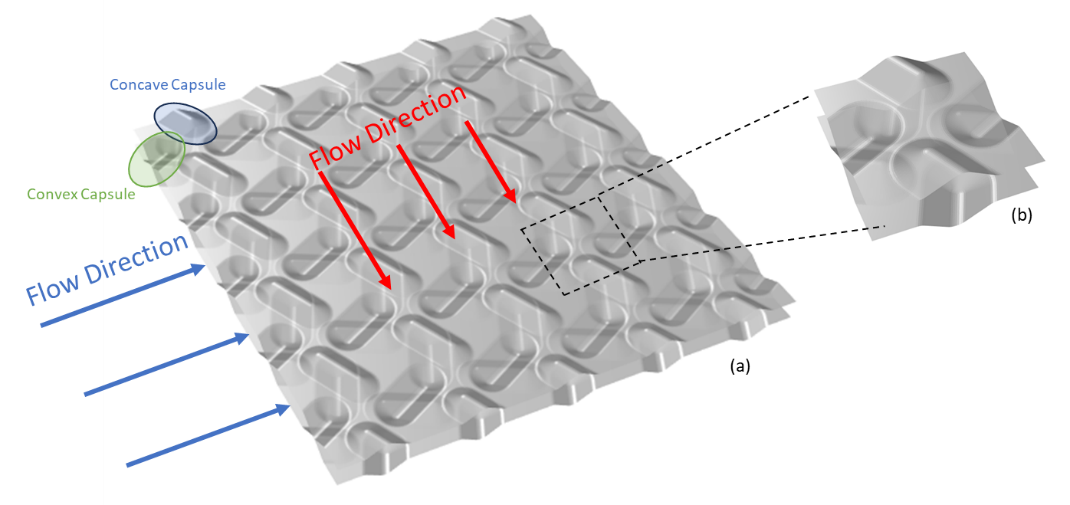
\includegraphics[width=0.9\textwidth]{media/image5.png}
  \caption{Schematics of capsule-type plate (a) and the unit cell (b).}
  \label{figure3}
\end{figure}

The major dimensions of the capsules are capsule length ($l$), capsule width ($w$), unit cell length ($l_c$), capsule height ($C_h$), and capsule angle ($\theta_c$). In which $l_c$ and $\theta_c$ can be derived from the equations $l_c=2\sqrt{(l/2)^2+(w/2)^2}$ and $|\theta_c|=\tan^{-1}((w/2)/(l/2))$, which yields only the magnitude of the capsule angle. The sign convention adopted in this study is as follows: $\theta_c > 0$ denotes a capsule whose major axis is rotated counterclockwise from the mainstream flow direction ($+x$), while $\theta_c < 0$ denotes a clockwise rotation. Accordingly, two neighboring plates carry capsules of equal magnitude but opposite sign (e.g., $+25$\degree\ and $-25$\degree), as described above. The center of the unit cell $C$ is at the intersection of two perpendicular lines connecting the touching points of the capsules and, together with $l_c$, $l$, and $w$, remains unchanged throughout the benchmarking conducted in this study. The dimensions of the initial CPHE geometry for this study are listed in Table~\ref{tab:dim-initial-cphe}.

\begin{figure}[H]
\centering
\begin{tabular}{cc}
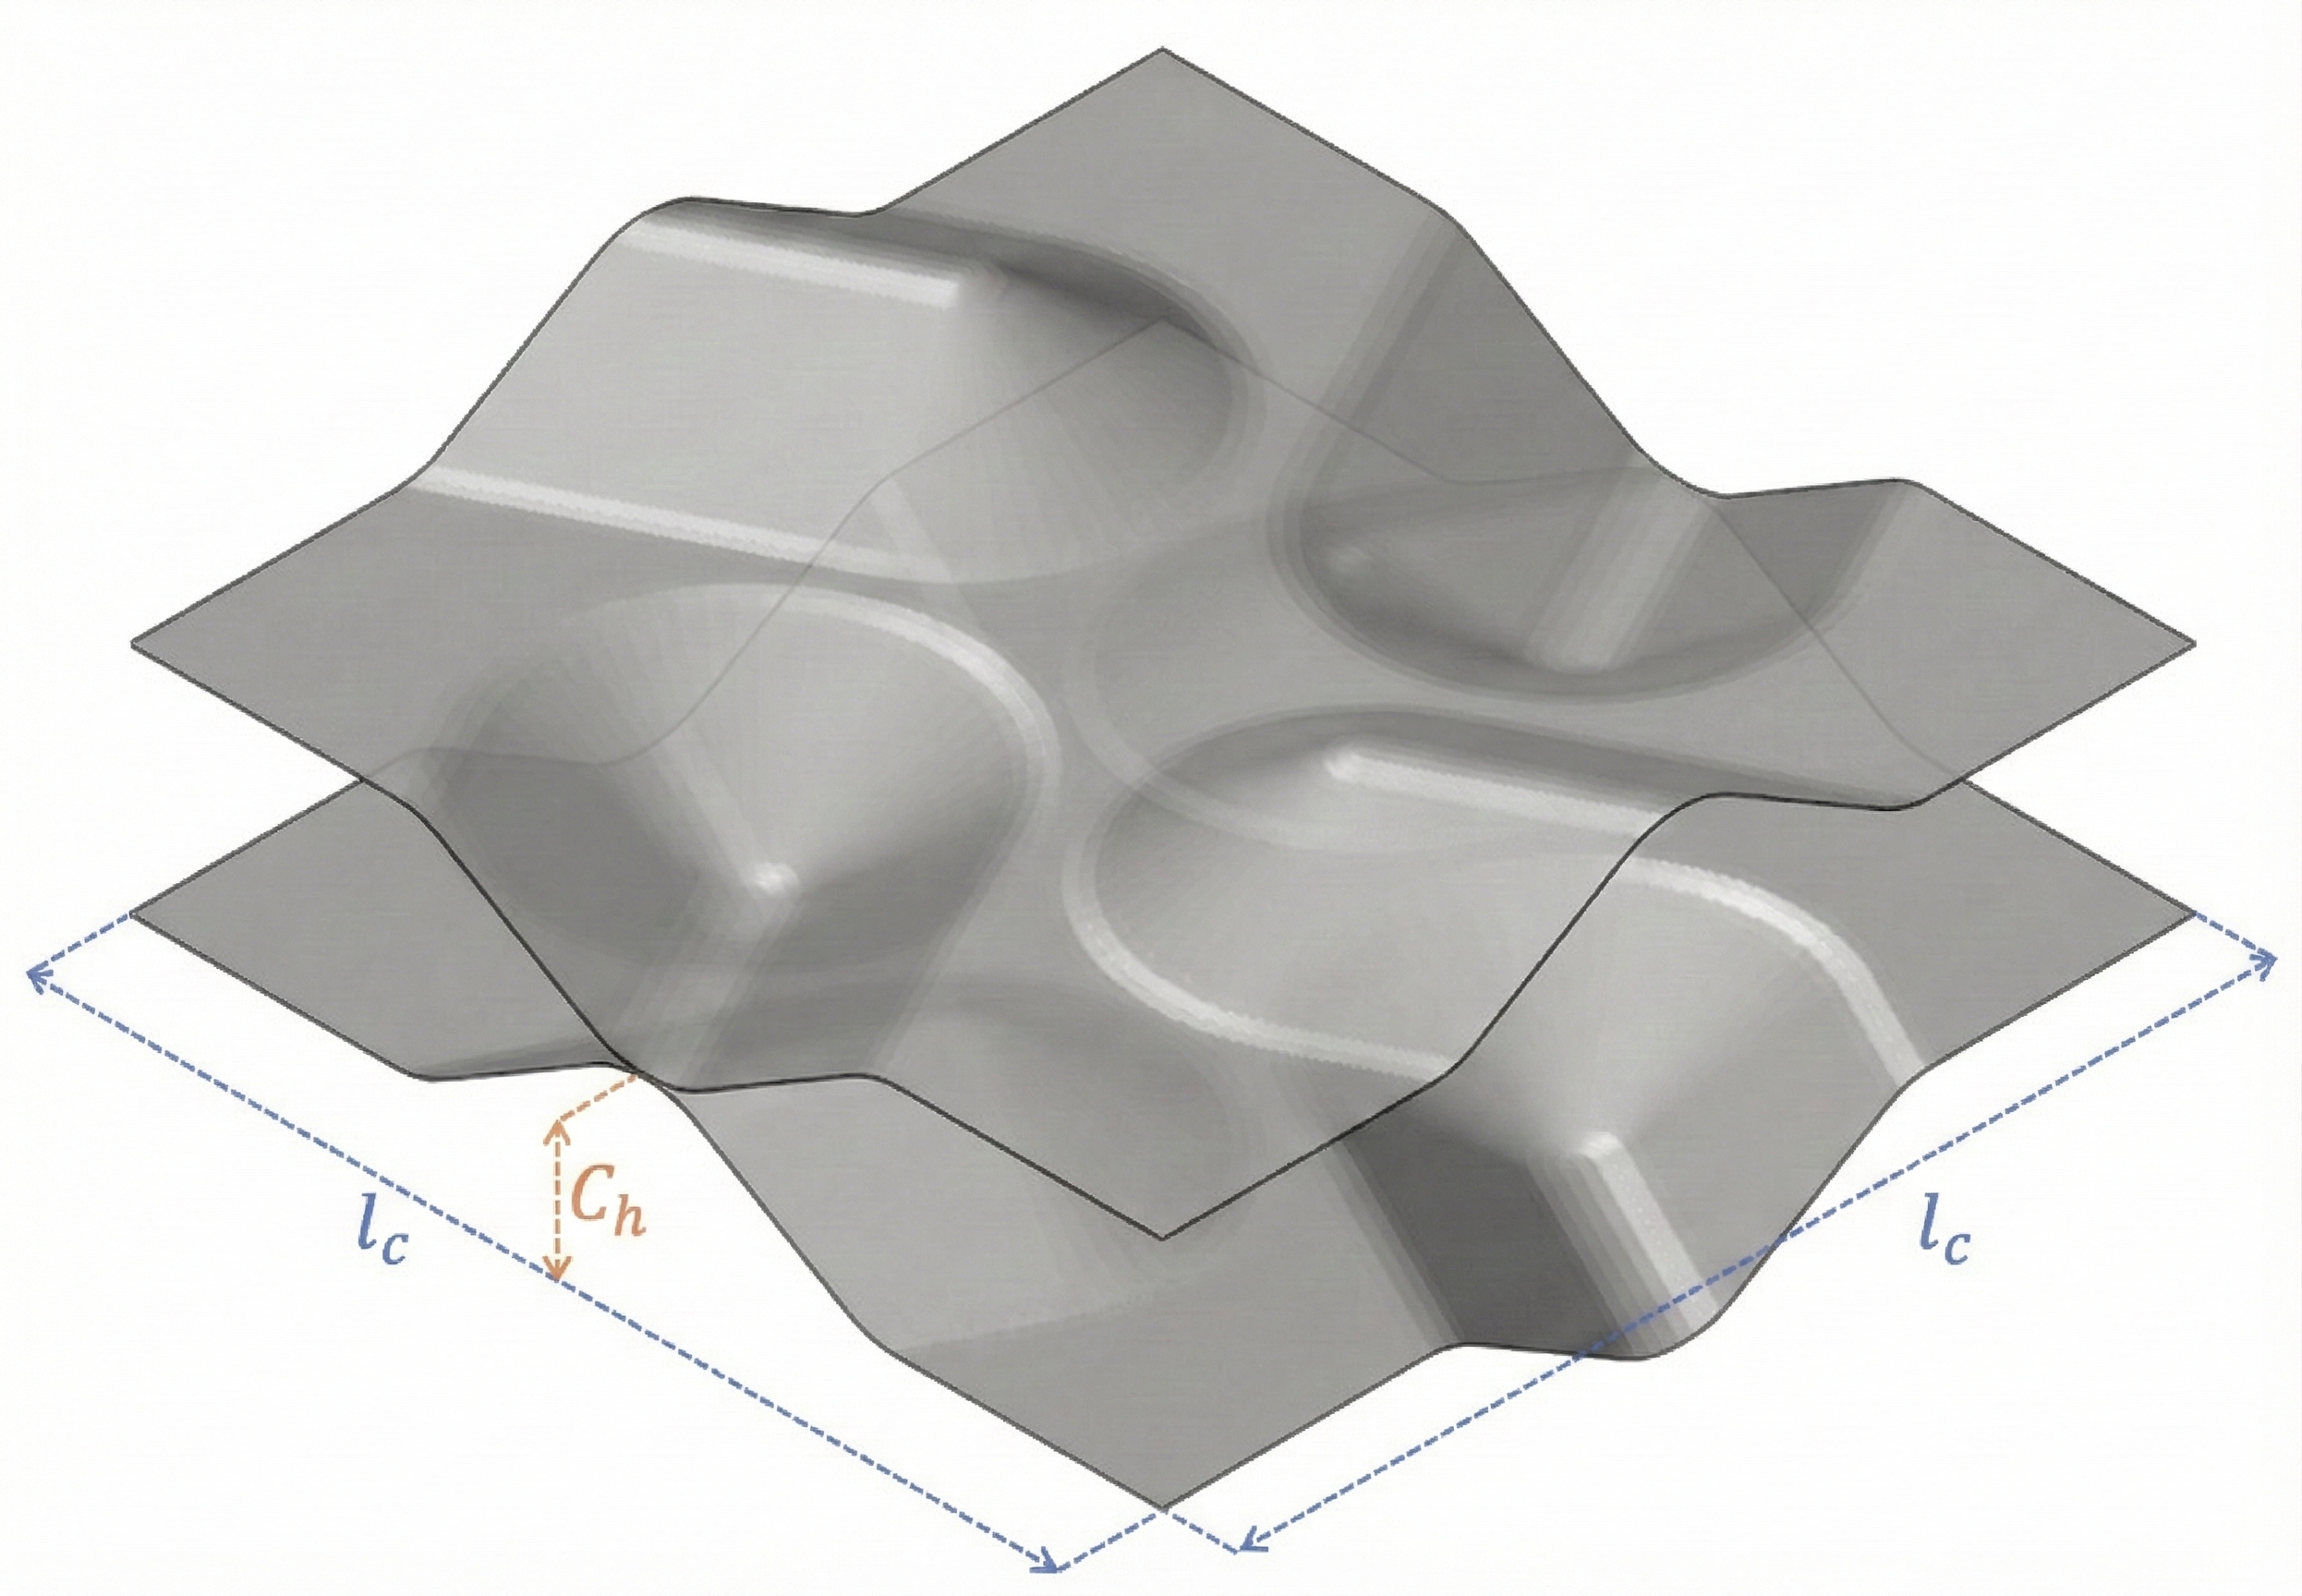
\includegraphics[width=0.425\textwidth]{media/image6.png} &
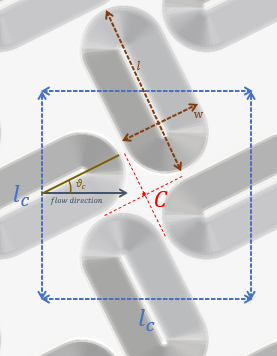
\includegraphics[width=0.2\textwidth]{media/image7.png} \\
\end{tabular}
\caption{Diagram explaining concept of CPHE unit cell.}
\label{figure4}
\end{figure}

\begin{table}[H]
\centering
\caption{Dimensions of the initial geometry---CPHE.}
\label{tab:dim-initial-cphe}
\renewcommand{\arraystretch}{1.3}
\begin{tabular}{lcccccc}
\hline
\textbf{Type} & $l$ (mm) & $w$ (mm) & $l_c$ (mm) & $C_h$ (mm) & $\theta_c$ (deg) \\
\hline
CPHE & 20 & 10 & 22.4 & 2.5 & 27\degree \\
\hline
\end{tabular}
\end{table}

\subsubsection{DPHE}
\label{sec:dphe_geometry}

Similar to CPHE, DPHEs consist of plates with a dimple embossing pattern, and embossing directions are opposing each other for neighboring plates. Fig.~\ref{figure5} shows the schematics of DPHE. The unit cell approach would also be applied in the DPHE study. Fig.~\ref{figure5} also shows the schematic drawing for DPHE and the associated unit cell for this study. The major dimensions of the dimples are dimple height ($D_h$), dimple spacing ($D_s$), and dimple diameter ($D$). Here $D_s$ is defined as the edge-to-edge gap between adjacent dimples. Defining the dimple pitch as $p = D + D_s$, the unit-cell length is $l_d = 2p = 2(D + D_s)$, so that $D_s = 0.5(l_d - 2D)$. For the initial study, $l_d = l_c = 22.4$~mm, giving $D_s = 0.5(22.4 - 2 \times 10) = 1.2$~mm. The summary of the dimensions of the initial geometry for DPHE is listed in Table~\ref{tab:dim-initial-dphe}.

\begin{figure}[H]
    \centering
    \begin{tabular}{cc}
    \begin{minipage}[t]{0.55\textwidth}
        \centering
        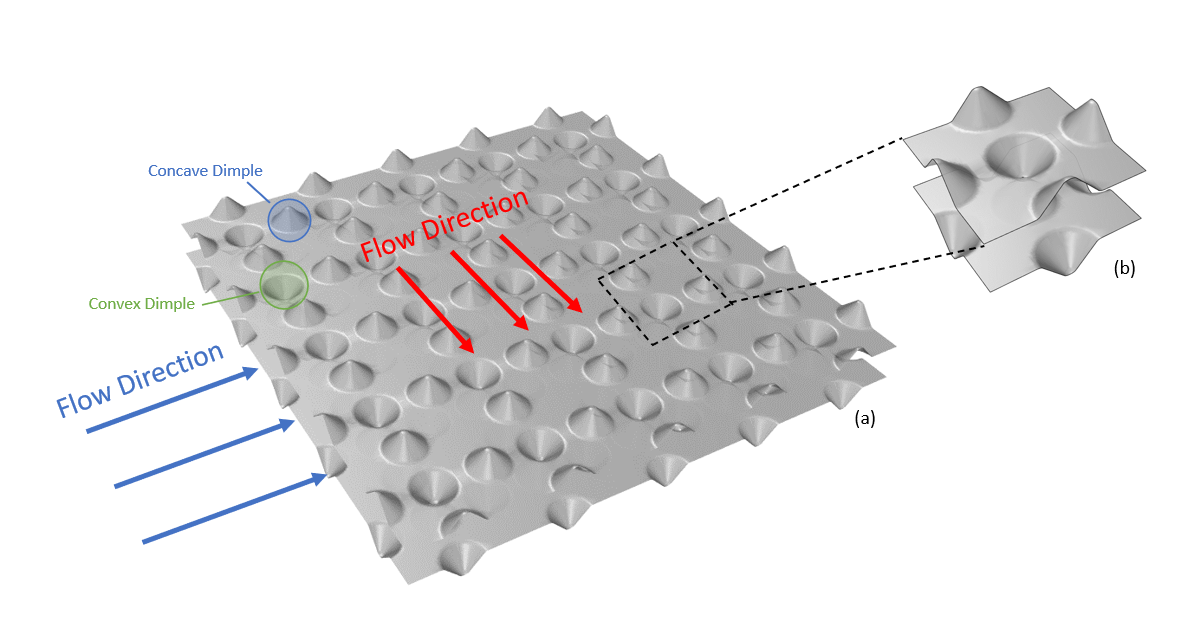
\includegraphics[width=\textwidth]{media/image8.png}
    \end{minipage} &
    \begin{minipage}[c]{0.3\textwidth}
        \centering
        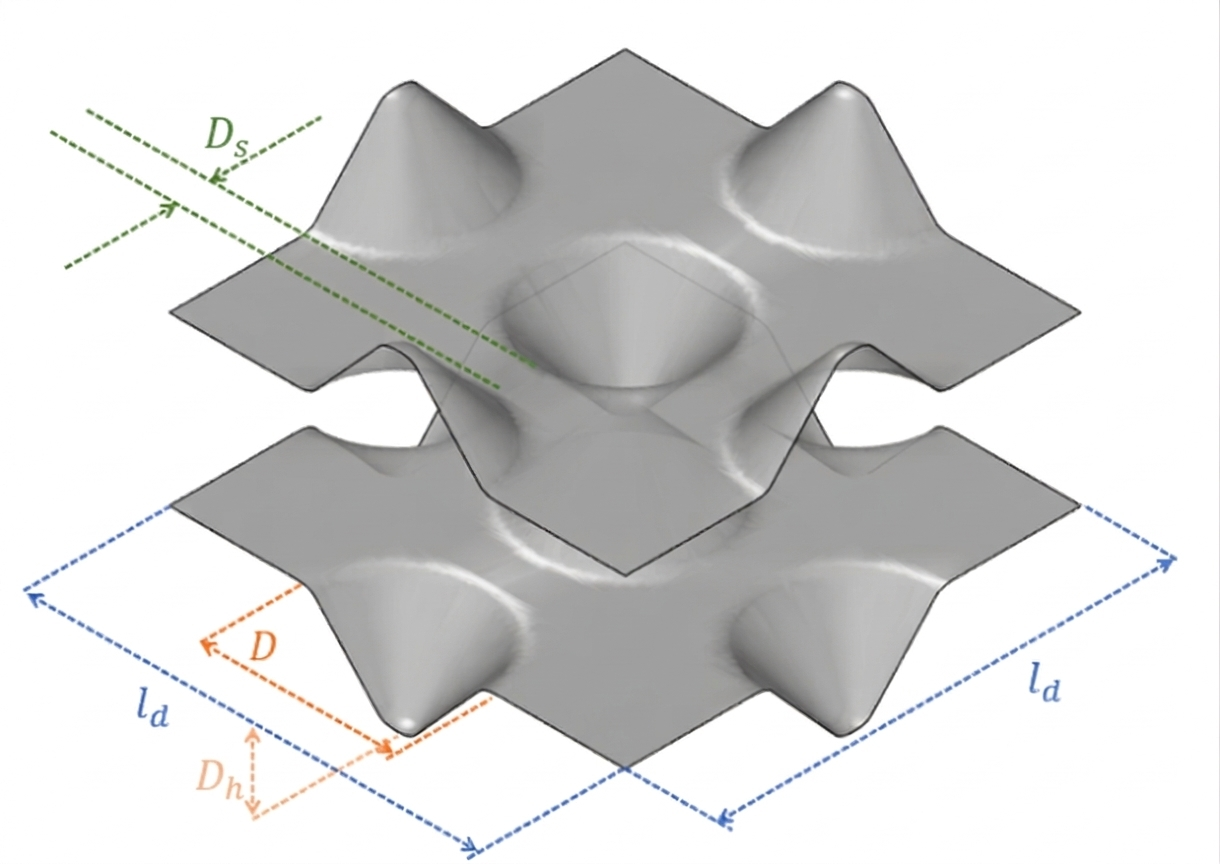
\includegraphics[width=\textwidth]{media/image9.png}
    \end{minipage}
    \end{tabular}
    \caption{Schematics of dimple-type plate (a) and the unit cell (b).}
    \label{figure5}
\end{figure}

\begin{table}[H]
\centering
\caption{Dimensions of the initial geometry---DPHE.}
\label{tab:dim-initial-dphe}
\renewcommand{\arraystretch}{1.3}
\begin{tabular}{lcccc}
\hline
\textbf{Type} & $D$ (mm) & $l_d$ (mm) & $D_h$ (mm) & $D_s$ (mm) \\
\hline
DPHE & 10 & 22.4 & 4 & 1.2 \\
\hline
\end{tabular}
\end{table}

\subsubsection{Periodic boundary}
\label{sec:periodic_boundary}

The flow within the computational domain consists of only one direction in the $x$-axis (single-phase flow). The flow parameters, such as velocity and kinetic turbulent energy of the inlet boundaries, are set by the outlet profile of the previous simulation, and the temperature is set as 293~K. When the pressure loss and heat transfer coefficient of the repeated simulations converge, it is considered that the flow and heat transfer are fully developed, the results are converged, and the data will be obtained for analysis. While there is no specific flow associated with span-wise direction ($y$-axis), a symmetry plane boundary condition is applied. In addition, the plates are set as a no-slip wall boundary condition with a constant wall temperature of 333~K, and the pressure outlet boundary condition is applied at the outlet plane ($x = l_c$), where $l_c = 22.4$~mm for all CPHE cases and for the DPHE dimple-height cases, while $l_c = 2(D + D_s)$ for the DPHE dimple-spacing cases (see Section~\ref{sec:dphe_geometry}). Reynolds number for the first simulation of all geometric parameters was set at 4282 based on \citet{jiang2019a}.

It should be noted that the Reynolds number is defined using the hydraulic diameter $D_e$ of the channel. The initial boundary condition for the first simulation of every parametric case prescribes the same inlet velocity, corresponding to Re\,=\,4282; in this sense, the starting Re is held constant across all geometries. However, because the iterative procedure feeds the converged outlet velocity profile back as the inlet for the next iteration, the velocity field evolves as the solution develops towards fully developed conditions. Consequently, the Reynolds number in the converged flow field will differ from the initial value, and this difference varies from geometry to geometry---no re-calibration of Re is performed between iterations. Crucially, the same convergence criterion was applied uniformly to all 27 cases: a simulation was deemed converged once the pressure drop and average heat transfer coefficient between successive iterations were equal or differed by a negligible amount. This consistent stopping rule ensures that, although the final Re varies with geometry, every reported data point represents a genuinely converged flow state obtained under identical procedural conditions.

\subsubsection{Geometric parameters}
\label{sec:geometric_parameters}

To understand the influence of geometric features on the thermo-hydraulic performance of Capsule-Type (CPHE) and Dimple-Type Plate Heat Exchangers (DPHE), a comprehensive parametric analysis is conducted. This analysis investigates the sensitivity of key performance metrics to changes in selected geometric parameters, specifically focusing on their impact on heat transfer enhancement and associated flow resistance. The parameters are chosen based on prior literature and their relevance in practical heat exchanger design \citep{hamedi2024, jiang2019, jiang2019a, jiang2020, soman2019, mocnik2024, jing2019}.

\paragraph{CPHE cases.}
Primary geometric variables are considered for CPHE:

\begin{itemize}
  \item \textbf{Capsule Angle} ($\theta_c$): The orientation of the capsule pattern relative to the main flow direction influences flow separation, vortex generation, and the formation of secondary flow structures. Varying this angle alters the flow interaction with the embossing features, potentially enhancing or suppressing turbulence. In this study, $\theta_c$ is varied from 12\degree\ to 42\degree\ in 5\degree\ increments, while all other geometric parameters are held constant. The selection of the capsule angle range from 12\degree\ to 42\degree\ effectively encompasses the majority of practical orientations for the capsule features relative to the main flow direction in PHEs. This range captures the key variations in flow interaction, such as vortex generation, flow separation, and turbulence enhancement, while allowing for a manageable unit cell size in the numerical simulations.

  \item \textbf{Capsule Height} ($C_h$): The height of the capsule embossing affects the cross-sectional area of the flow channel, altering the local velocity gradients and promoting different levels of shear and mixing. With reference to the industrial norm of press depth for chevron plates of 2.5 to 4~mm \citep{laval2022}, capsule heights ranging from 2~mm to 5~mm are investigated in 0.5~mm increments.
\end{itemize}

For each configuration, steady-state CFD simulations are performed under identical boundary conditions. Key thermofluid parameters such as Nusselt number (Nu), pressure drop ($\Delta p$), and turbulence kinetic energy (TKE) distributions are evaluated to assess the trade-off between heat transfer enhancement and hydraulic performance.

\paragraph{DPHE cases.}
For DPHE, which utilizes rounded-conical dimple patterns, the following parameters are varied:

\begin{itemize}
  \item \textbf{Dimple Height} ($D_h$): The embossing depth influences the intensity and persistence of vortex structures within the flow. Change in height affects the strength of recirculating zones and shear layers. Similar to capsules, heights ranging from 2~mm to 5~mm are investigated in increments of 0.5~mm.

  \item \textbf{Dimple Spacing} ($D_s$): Defined as the edge-to-edge gap between adjacent dimples (see Section~\ref{sec:dphe_geometry}), spacing controls the interaction between neighboring wake regions. Closely spaced dimples tend to increase cumulative turbulence, while wider spacing separates wake regions and may reduce mixing. In this study, $D_s$ is varied from 1.2~mm to 11.2~mm in increments of 2~mm. The dimple diameter ($D$) is kept constant to isolate spacing effects. This range covers spacing where vortex interactions transition from merged to isolated wakes as observed in various CFD and experimental studies investigating dimple arrays on heat transfer surfaces \citep{oo2019, falih2024}, capturing the trade-off between turbulence intensity and hydraulic performance for practical design benchmarking.
\end{itemize}

Each DPHE variation is evaluated using the same simulation setup as described for CPHE to maintain consistency in the analysis approach. Performance is quantified in terms of both thermal and hydraulic effectiveness.

\paragraph{Relative Embossing Depth (RED).}
To plot all 27 parametric cases on a single geometric axis, a unified dimensionless parameter is needed. Because each parameter family modifies the channel cross-section differently---capsule angle changes the orientation of the embossing, whereas capsule height, dimple height, and dimple spacing change linear dimensions---no single raw geometric variable is directly comparable across families. The Relative Embossing Depth is therefore defined as
\begin{equation}
\text{RED} = \frac{h}{D_e}
\label{eq:red}
\end{equation}
where $h$ is the embossing height of the feature ($C_h$ for capsule cases, $D_h$ for dimple cases) and $D_e$ is the hydraulic diameter of the corresponding channel (Eq.~\eqref{eq:De}). For capsule-angle cases, $h$ is the fixed capsule height (2.5~mm), but $D_e$ changes with angle because of the unit-cell geometry---and therefore the inlet area $A_0$ and heat-transfer surface $S$---varies with $\theta_c$. Similarly, for dimple-spacing cases, $h$ is the fixed dimple height (4~mm), while $D_e$ changes with spacing. RED therefore captures the fact that every geometric modification ultimately alters the ratio of embossing protrusion to effective channel size, regardless of whether the varied parameter is an angle, a height, or a spacing.

It should be noted that RED is a derived quantity: recovering the specific geometric case from a given RED value requires knowledge of the corresponding $D_e$, which in turn depends on the full unit-cell geometry (Eq.~\eqref{eq:De}). The individual $D_e$ values are not tabulated in this study; however, because each parametric family varies only one geometric variable at a time, the mapping from RED back to the physical parameter is unambiguous within each family.

\subsubsection{Performance evaluation criteria}
\label{sec:performance_criteria}

The following performance metrics are used to compare the results:

\begin{itemize}
  \item \textbf{Nusselt Number} (Nu): Indicates the convective heat transfer relative to conductive heat transfer across the fluid layer. A higher Nu implies better heat transfer enhancement.

  \item \textbf{Fanning Friction Factor} ($f$): Measures flow resistance, directly related to the pressure drop across the heat exchanger.

  \item \textbf{Thermal Performance Factor} (TPF): To enable a direct, cross-family ranking of all parametric cases on a single scale, the thermal performance factor is adopted:
  \begin{equation}
  \text{TPF} = \frac{\text{Nu}}{f^{1/3}}
  \label{eq:tpf}
  \end{equation}
  This metric quantifies the convective heat-transfer gain (Nu) per unit of flow-resistance penalty ($f^{1/3}$), where the one-third exponent arises from the fact that pumping power scales with $f$ while heat transfer scales with Nu, making Nu/$f^{1/3}$ a relative indicator of thermo-hydraulic merit. Because the iterative convergence procedure described in Section~\ref{sec:periodic_boundary} allows the final Reynolds number to differ from geometry to geometry, the TPF values reported here should be interpreted as a relative performance index evaluated at each case's own converged operating state, rather than a strict equal-pumping-power or equal-duty comparison. Notwithstanding this caveat, TPF remains a useful ranking metric: it requires no auxiliary geometric parameter and therefore places capsule-angle, capsule-height, dimple-height, and dimple-spacing cases on a consistent thermo-hydraulic scale. A higher TPF indicates a more favorable balance between heat transfer and flow resistance. Sections~\ref{sec:disc_capsule_angle}--\ref{sec:disc_dimple_spacing} analyze trends in Nu and $f$ individually; Section~\ref{sec:tgg_comparison} uses TPF to rank all cases and compare both embossing families.
\end{itemize}

Performance trends are analyzed to identify optimal geometries that provide maximum thermal enhancement with acceptable frictional losses. Results are compared across geometries to determine the most effective embossing configurations for enhancing the heat exchanger's efficiency.

\begin{table}[H]
\centering
\caption{Geometric parameter cases for CPHE and DPHE.}
\label{tab:geom_cases}
\footnotesize
\renewcommand{\arraystretch}{1.2}
\begin{tabularx}{\textwidth}{ll>{\raggedright\arraybackslash}l>{\raggedright\arraybackslash}X}
\hline
\textbf{Heat Exchanger Type} & \textbf{Parameter} & \textbf{Cases} & \textbf{Description} \\ \hline
\multirow{2}{*}{CPHE (Capsule-Type)} 
& Capsule Angle ($\theta_c$) & 12\degree--42\degree & Orientation of capsule pattern relative to main flow direction with 5\degree\ increments and a capsule height of 2.5~mm. \\
& Capsule Height ($C_h$) & 2--5~mm & Height of capsule embossing feature with 0.5~mm increments and a capsule angle of 27\degree. \\ \hline
\multirow{2}{*}{DPHE (Dimple-Type)} 
& Dimple Height ($D_h$) & 2--5~mm & Height of the dimple embossing feature with 0.5~mm increments and a dimple spacing of 1.2~mm. \\
& Dimple Spacing ($D_s$) & 1.2--11.2~mm & Edge-to-edge distance between dimples with 2~mm increments and a dimple height of 4~mm. \\ \hline
\end{tabularx}
\end{table}

\subsection{Mesh independence}
\label{sec:mesh}

An unstructured poly-hexacore mesh type is adopted for the mesh generation. Certain criteria are set for the mesh generated to minimize discretization and interpolation error \citep{sorgente2023, juretic2010}, including mesh orthogonality and mesh skewness. For this study, the criteria of minimum mesh orthogonality of 0.1 and maximum mesh skewness of 0.8 are set for all cases.

To accurately predict the wall heat transfer coefficient and the wall shear stress close to the wall, prism layers are included in the mesh generation. Prism layers are hexahedral cells that are normal to the wall boundary to capture the steep normal gradient in the mean velocity and temperature inside the thermal and hydraulic boundary layers. The total prism layer thickness should capture the turbulent boundary layer of the flow. The initial estimation of the total boundary layer thickness $\delta$ can be deducted through the following equation: $\delta/x = 0.16/\text{Re}_x^{1/7}$ \citep{cengel2014}, where $x$ is the total stream length, which is $l_c$ and $l_d$ for this study, and Re is the Reynolds number.

For the prism layers to accurately predict the near-wall behavior, the first prism layer thickness (or the first layer height) plays an important role in calculating the behavior at the viscous sub-layer, as it is related to $y^+$, which is a dimensionless distance normal to the wall, and the near-wall kinematic viscosity can be calculated accordingly. As suggested by \citet{eca2018}, to minimize the numerical uncertainty, $y^+$ near 0.1 should be applied for the SST $k$--$\omega$ turbulence model; therefore, the first layer height is set to 0.0002~mm, and the resultant $y^+$ is 0.087---see Fig.~\ref{figure6}.

\begin{figure}[H]
  \centering
  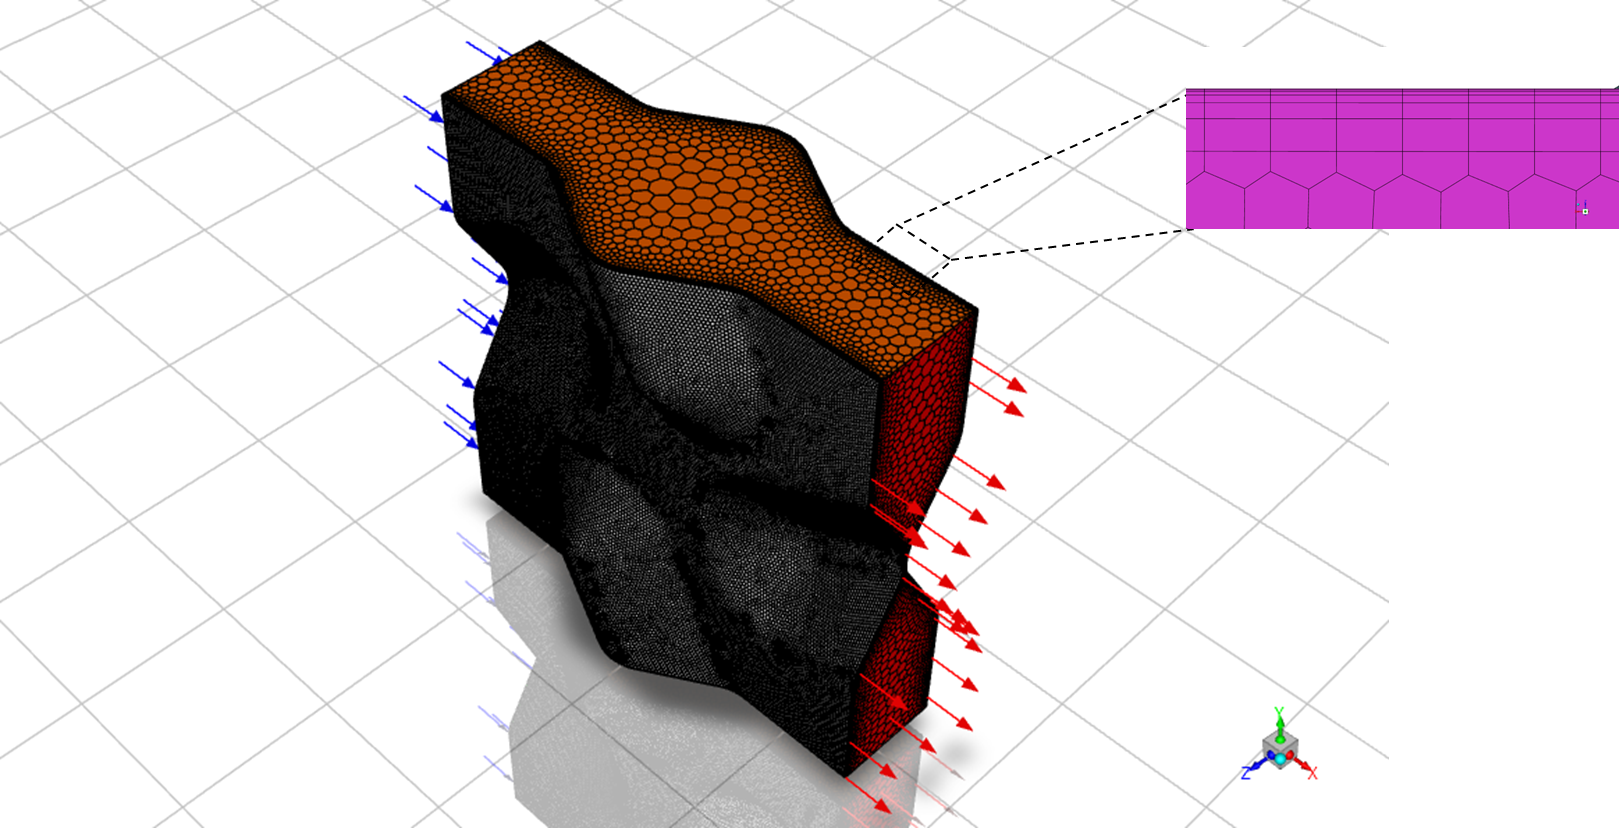
\includegraphics[width=0.7\textwidth]{media/Picture4.png}
  \caption{First layer height of 0.0002~mm and $y^+$(max) of 0.0871.}
  \label{figure6}
\end{figure}

The flow velocity and turbulence kinetic energy of the outlet profile will be set as the inlet boundary. For this approach, the mesh of the inlet and outlet boundaries must be identical for accurate pairing of data. Periodic meshing will be applied during mesh generation for this purpose, and the boundaries will be redefined as stated in Section~\ref{sec:periodic_boundary} in the pre-calculation phase.

A mesh independence study is performed for CPHE with $h = 2.5$~mm, as shown in Fig.~\ref{figure7}. $f$ and Nu for five different meshes ranging from $\sim$100k to $\sim$1.1M elements are compared to determine the best coarsest mesh. The difference of $f$ and Nu between the results of $\sim$600k mesh count and $\sim$1.1M mesh count is less than 2.7\% and 2\%, respectively, showing the results obtained from $\sim$600k mesh count are reliable and validated, and will be employed in this study.

\begin{figure}[H]
  \centering
  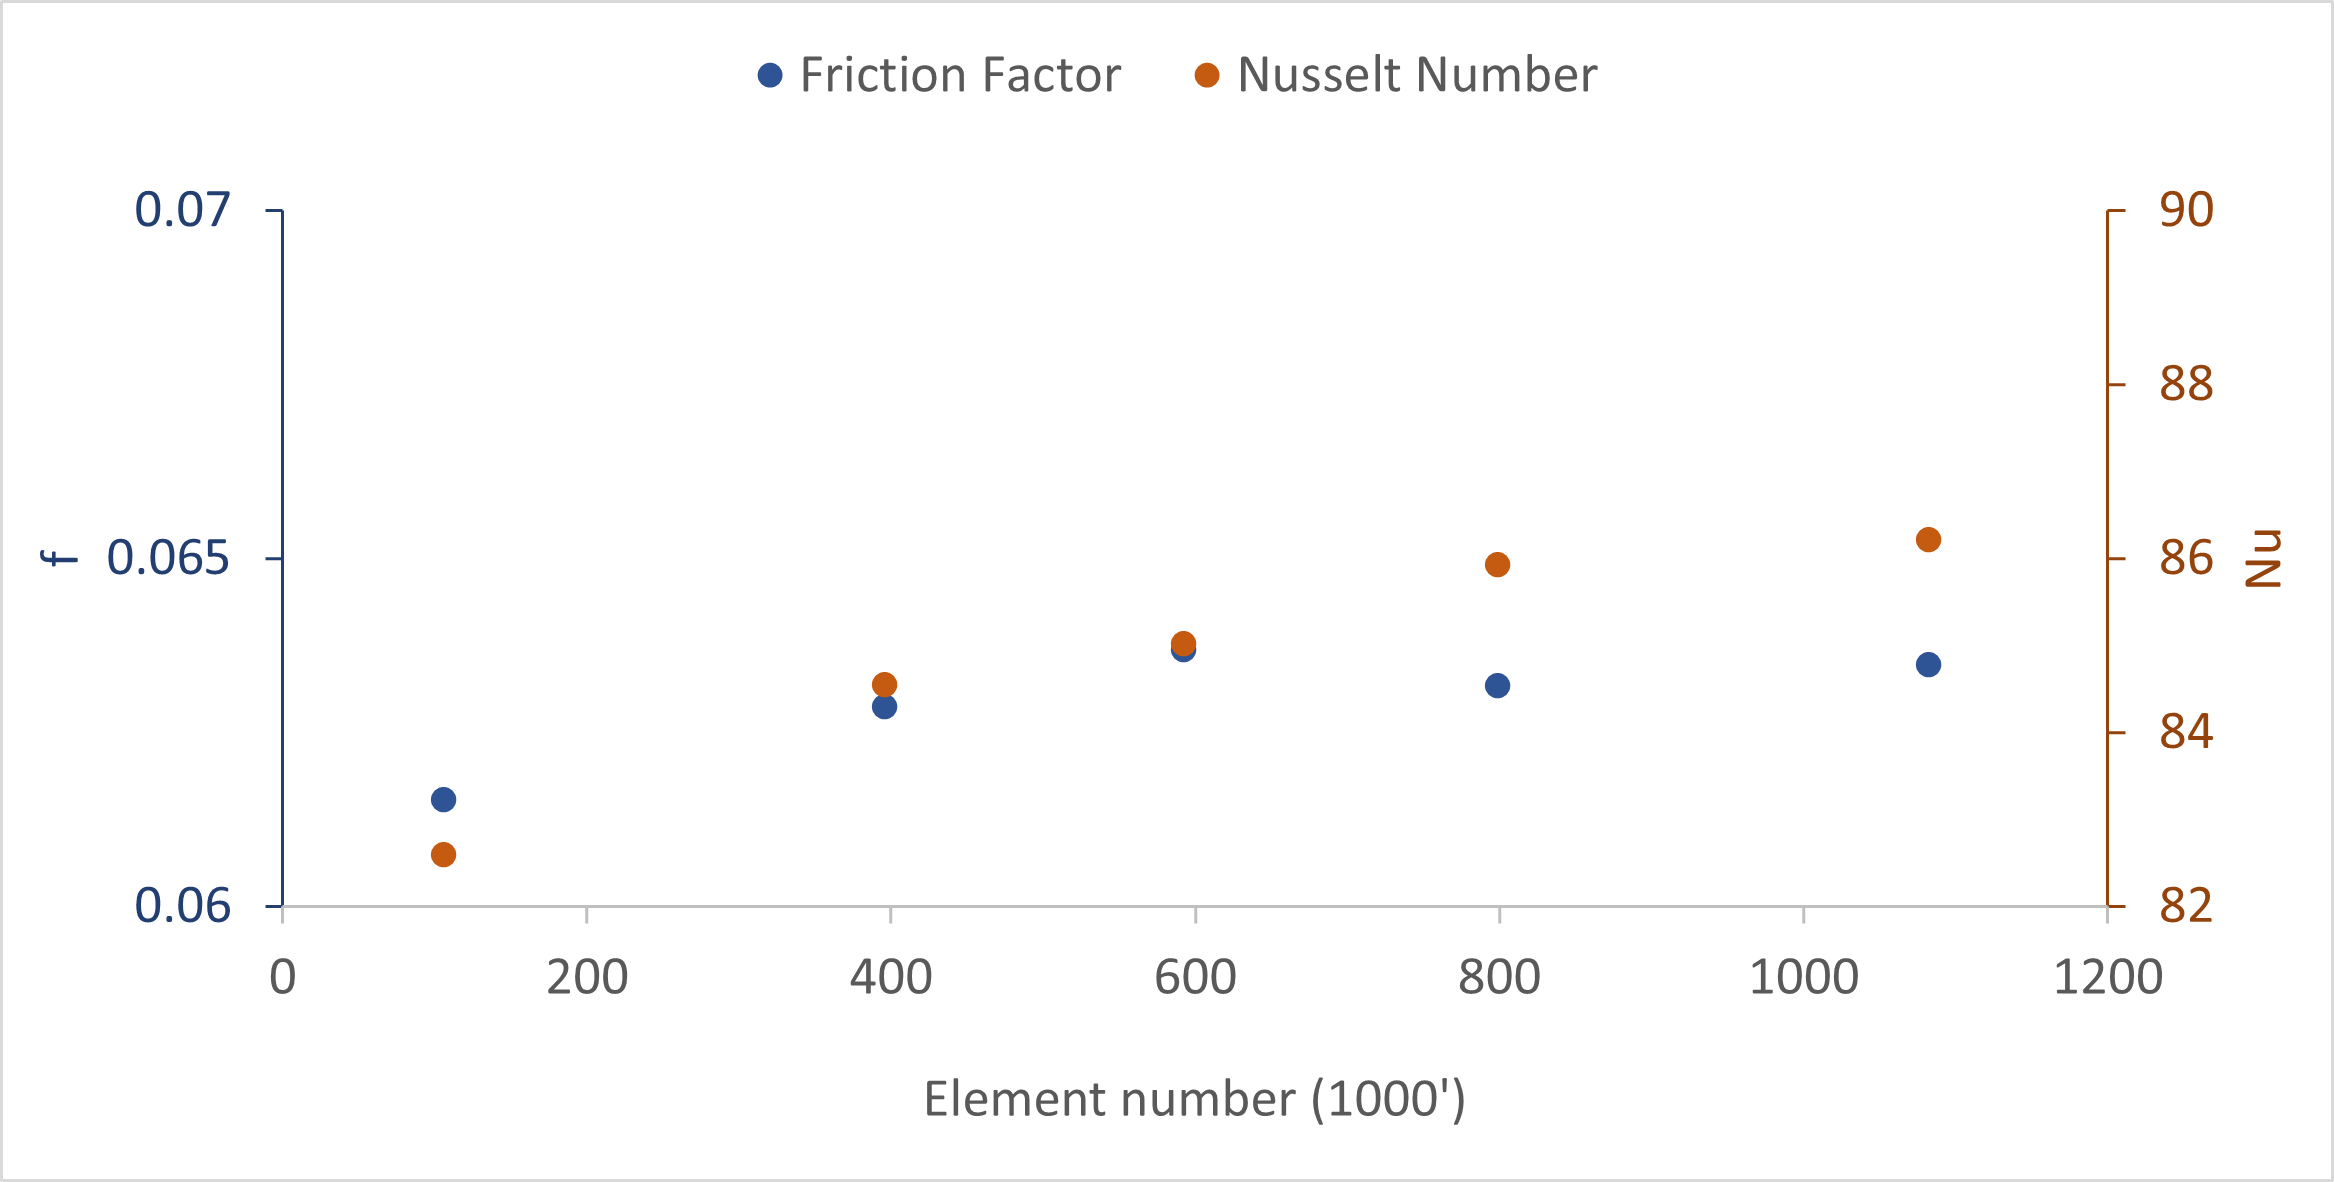
\includegraphics[width=0.7\textwidth, trim={7 5 10 5}, clip]{media/image10_v1.png}
  \caption{Mesh independence study---element number.}
  \label{figure7}
\end{figure}

\section{Results}
\label{sec:results}

The numerical simulations conducted in this study provide detailed insight into the thermo-hydraulic behavior of capsule-type and dimple-type plate heat exchangers under a variety of geometric configurations. By examining the influence of selected design parameters---namely the capsule angle and height in CPHE, and the dimple height and spacing in DPHE---the impact on flow structures, pressure drop, and heat transfer performance is assessed. Key fluid dynamic behaviors, including vortex generation, turbulence intensity, and recirculating flow patterns, are visualized through turbulence kinetic energy contours and streamline plots. Temperature distributions further reveal the relationship between geometric enhancements and thermal mixing. These findings enable the identification of design trends that balance improved heat transfer effectiveness with manageable pressure penalties, supporting the development of more efficient compact heat exchanger designs.

\subsection{CPHE parametric study}
\label{sec:cphe_results}

Two major improvements or modifications are proposed in this study to investigate the impact on the pressure drop and heat transfer rate: 1) the angle between the capsule and the mainstream; 2) the capsule height.

\subsubsection{Capsule angle}
\label{sec:capsule_angle_results}

The angle between the capsule and the mainstream flow direction would greatly affect the flow field, which would vary the turbulent behavior and ultimately alter the performance of the pressure drop and heat transfer. Eddies are the major heat transfer mechanism within CPHE due to the nature of mixing heated fluid (from near wall boundaries due to convection) with cold fluid, which improves the exchange of fluid particles between different flow regions with minimal increases in pressure loss \citep{jacobi1995}. To investigate the performance of these heat exchangers, turbulence kinetic energy (TKE) contour plot at the middle $z$-axis section (Fig.~\ref{figure8}), and two-dimensional streamlines (Fig.~\ref{figure9}) are plotted. It is found that TKE distribution within the channel is comparatively more uniform and lower for lower $\theta_c$ (i.e., Fig.~\ref{figure8}a) than higher $\theta_c$ (i.e., Fig.~\ref{figure8}f \& g), while TKE represents the mean kinetic energy per unit mass in the fluctuating velocity field \citep{pope2000}. Note that RANS predicts a time-averaged solution; the irregular contour shown in Figs.~\ref{figure8}e, f, and g indicates a fluctuation in the time-averaged means, which ultimately shows that there is less magnitude and fluctuation in energy associated with eddies locally and in the whole computational domain for lower $\theta_c$.

\begin{figure}[H]
    \centering
    \resizebox{\textwidth}{!}{%
    \renewcommand{\arraystretch}{1.0}
    \begin{tabular}{ccccc}
        \multirow{2}{*}{
            \begin{minipage}[c]{0.14\textwidth}
                \centering
                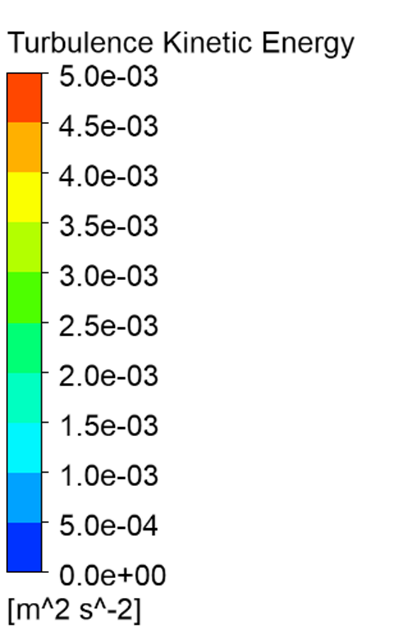
\includegraphics[width=\linewidth]{media/image50.png}
            \end{minipage}
        } &
        \begin{minipage}[t]{0.17\textwidth}
            \centering
            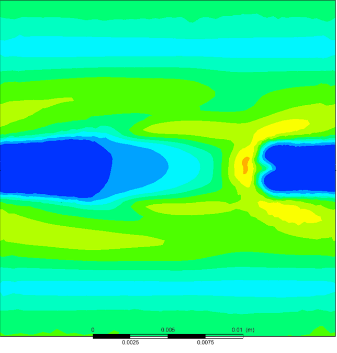
\includegraphics[width=\textwidth]{media/image17.png}\\
            \vspace{-1em}
            {\scriptsize\textbf{(a) $\theta_c$ = 12\degree}}
        \end{minipage} &
        \begin{minipage}[t]{0.17\textwidth}
            \centering
            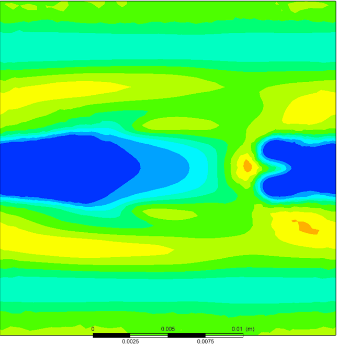
\includegraphics[width=\textwidth]{media/image19.png}\\
            \vspace{-1em}
            {\scriptsize\textbf{(b) $\theta_c$ = 17\degree}}
        \end{minipage} &
        \begin{minipage}[t]{0.17\textwidth}
            \centering
            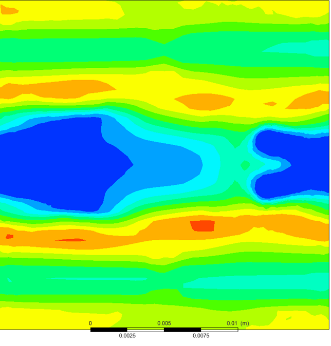
\includegraphics[width=\textwidth]{media/image20.png}\\
            \vspace{-1em}
            {\scriptsize\textbf{(c) $\theta_c$ = 22\degree}}
        \end{minipage} &
        \begin{minipage}[t]{0.17\textwidth}
            \centering
            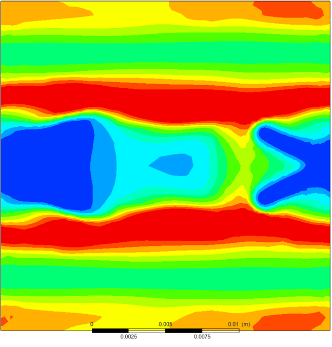
\includegraphics[width=\textwidth]{media/image21.png}\\
            \vspace{-1em}
            {\scriptsize\textbf{(d) $\theta_c$ = 27\degree}}
        \end{minipage} \\
         &\begin{minipage}[t]{0.17\textwidth}
            \centering
            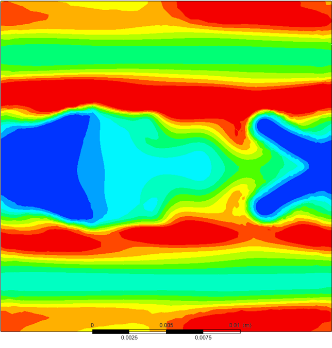
\includegraphics[width=\textwidth]{media/image22.png}\\
            \vspace{-1em}
            {\scriptsize\textbf{(e) $\theta_c$ = 32\degree}}
        \end{minipage} &
        \begin{minipage}[t]{0.17\textwidth}
            \centering
            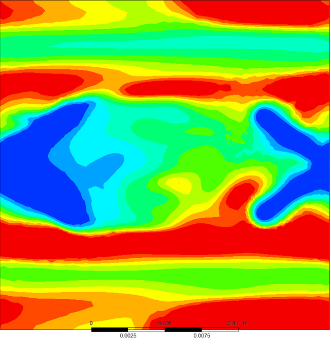
\includegraphics[width=\textwidth]{media/image23.png}\\
            \vspace{-1em}
            {\scriptsize\textbf{(f) $\theta_c$ = 37\degree}}
        \end{minipage} &
        \begin{minipage}[t]{0.17\textwidth}
            \centering
            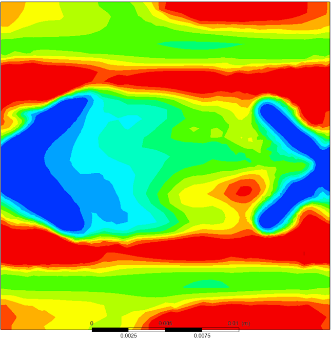
\includegraphics[width=\textwidth]{media/image24.png}\\
            \vspace{-1em}
            {\scriptsize\textbf{(g) $\theta_c$ = 42\degree}}
        \end{minipage} & \\
    \end{tabular}%
    }
    \caption{TKE distribution of middle $z$-axis section of CPHE with various $\theta_c$.}
    \label{figure8}
\end{figure}

\begin{figure}[H]
    \centering
    \resizebox{\textwidth}{!}{%
    \renewcommand{\arraystretch}{1.1}
    \begin{tabular}{cccc}
        \begin{minipage}[t]{0.2\textwidth}
            \centering
            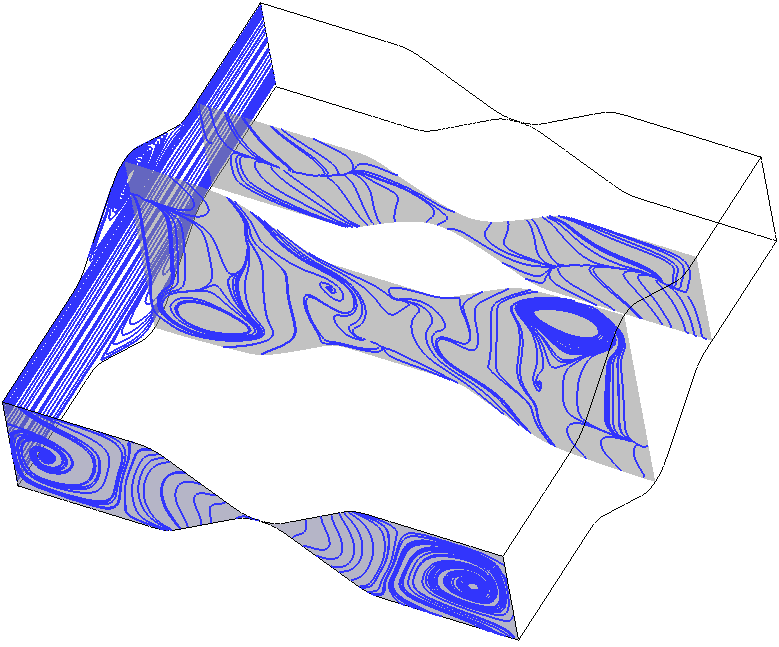
\includegraphics[width=\textwidth]{media/2D_stream_CA_12.png}
            {\scriptsize\textbf{(a) $\theta_c$ = 12\degree}}
        \end{minipage} &
        \begin{minipage}[t]{0.2\textwidth}
            \centering
            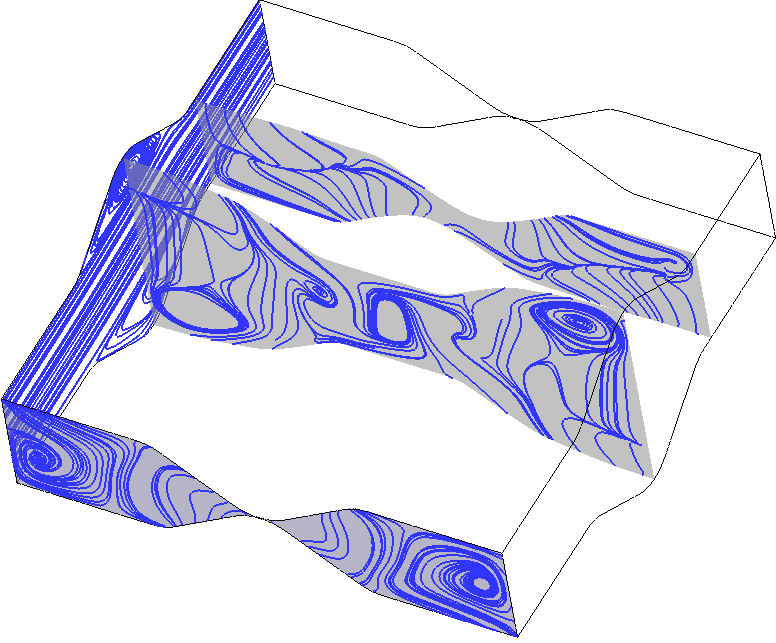
\includegraphics[width=\textwidth]{media/2D_stream_CA_17.png}
            {\scriptsize\textbf{(b) $\theta_c$ = 17\degree}}
        \end{minipage} &
        \begin{minipage}[t]{0.2\textwidth}
            \centering
            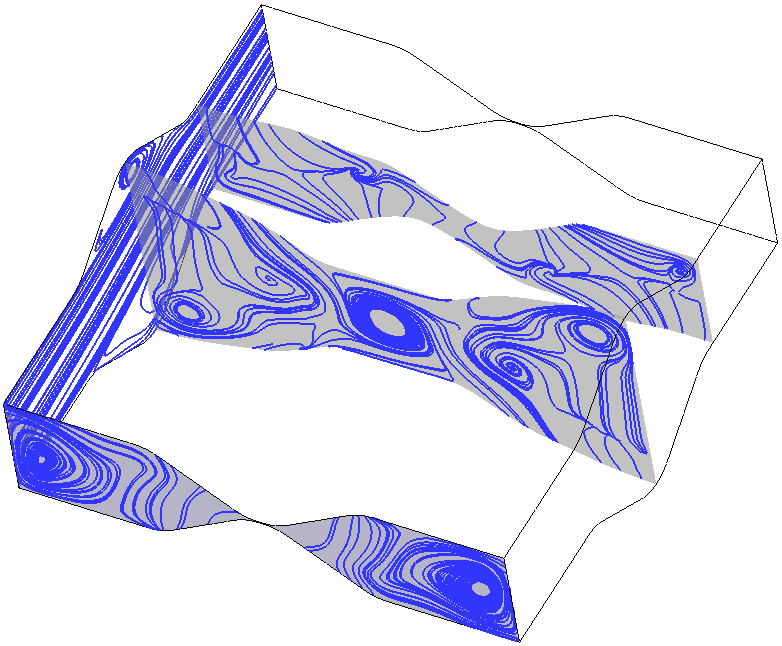
\includegraphics[width=\textwidth]{media/2D_stream_CA_22.png}
            {\scriptsize\textbf{(c) $\theta_c$ = 22\degree}}
        \end{minipage} &
        \begin{minipage}[t]{0.2\textwidth}
            \centering
            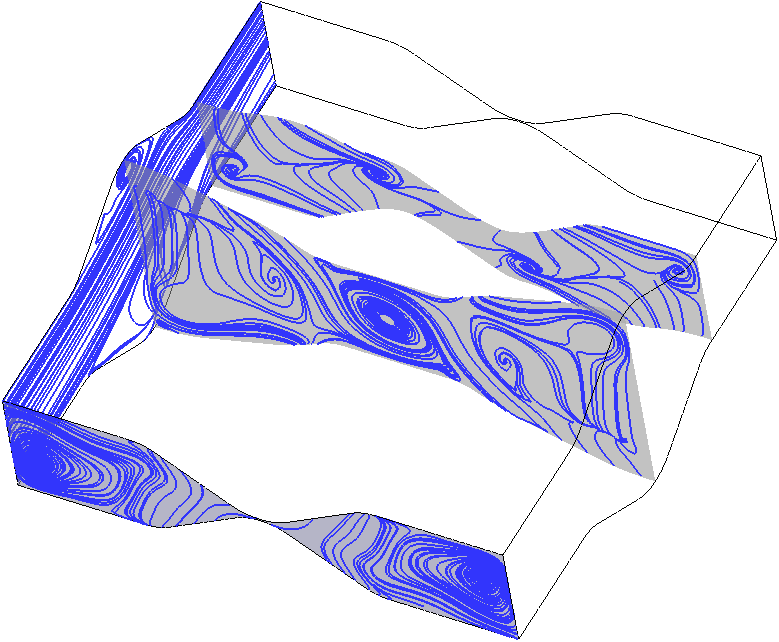
\includegraphics[width=\textwidth]{media/2D_stream_CA_27.png}
            {\scriptsize\textbf{(d) $\theta_c$ = 27\degree}}
        \end{minipage} \\
        \begin{minipage}[t]{0.2\textwidth}
            \centering
            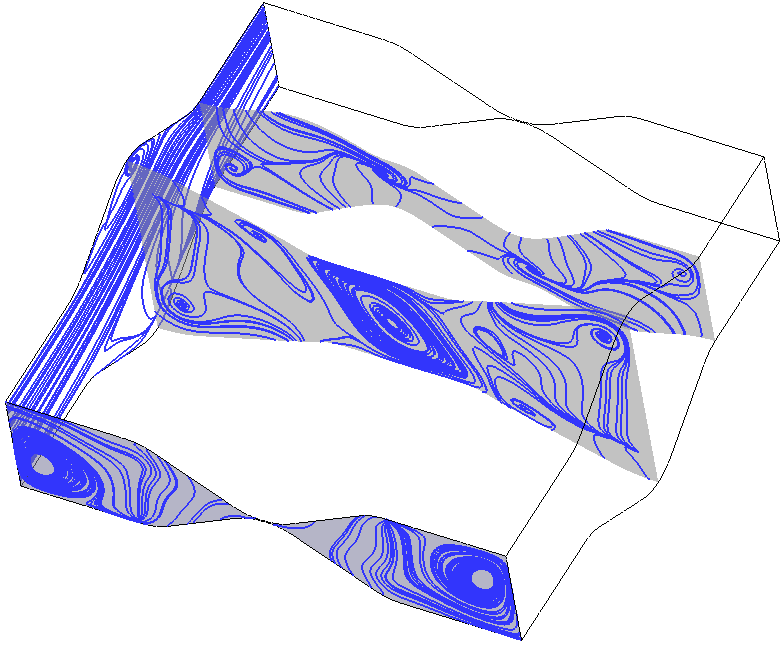
\includegraphics[width=\textwidth]{media/2D_stream_CA_32.png}
            {\scriptsize\textbf{(e) $\theta_c$ = 32\degree}}
        \end{minipage} &
        \begin{minipage}[t]{0.2\textwidth}
            \centering
            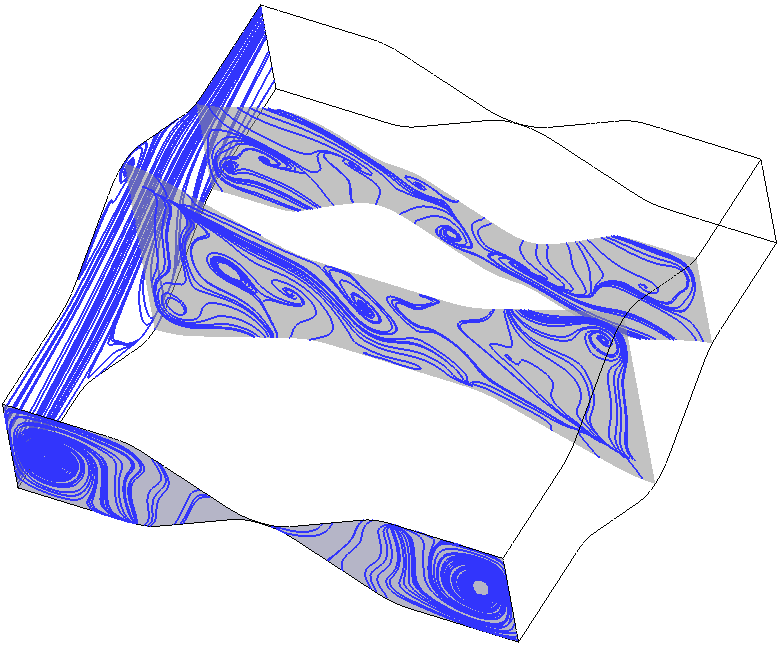
\includegraphics[width=\textwidth]{media/2D_stream_CA_37.png}
            {\scriptsize\textbf{(f) $\theta_c$ = 37\degree}}
        \end{minipage} &
    \begin{minipage}[t]{0.2\textwidth}
        \centering
        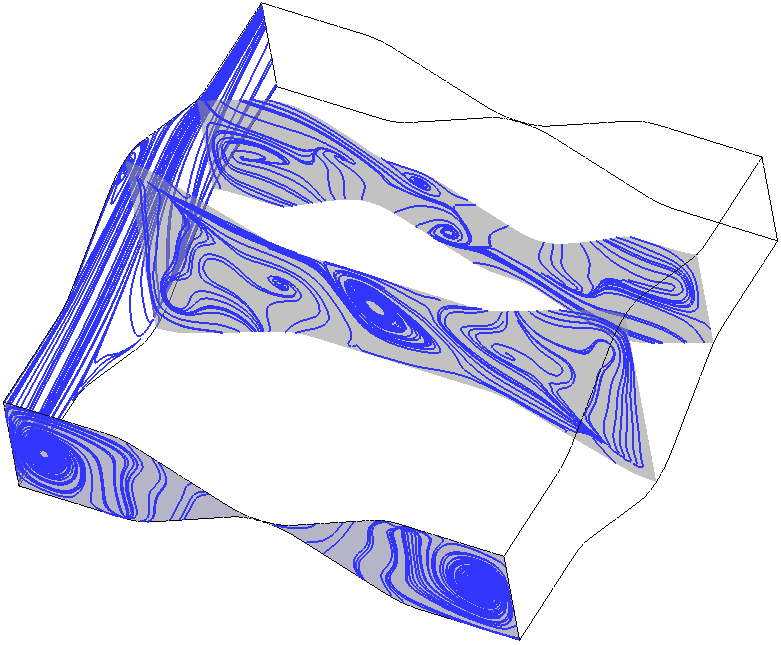
\includegraphics[width=\textwidth]{media/2D_stream_CA_42.png}
        {\scriptsize\textbf{(g) $\theta_c$ = 42\degree}}
    \end{minipage} &
     \begin{minipage}[t]{0.2\textwidth}
        \centering
        
\includegraphics[width=\textwidth]{media/Screenshot_2025-08-01_205019.png}
    \end{minipage} \\
    \end{tabular}%
    }
    \caption{2D streamlines of CPHE with various $\theta_c$.}
    \label{figure9}
\end{figure}

To further analyze the flow characteristics, the vortex pattern is investigated with 2D and 3D streamlines (Fig.~\ref{figure9}). 2D streamlines are visualized at planes located at $x = 0$, $x = l_c/2$, and $x = 3l_c/4$. When $\theta_c$ is low, wake vortices are generated behind the convex capsule in the stream-wise direction, which is located in the middle of the computational domain, causing lower pressure and recirculating flow. Recirculating flow can also be found in the concave capsules in the spanwise direction due to the expansion of cross-sectional area along the middle $x$-axis. While for higher $\theta_c$, the wake region is disturbed due to the reattachment of the flow after being redirected by the convex capsules, the disturbance enhances the turbulence and introduces more small eddies, which perform better than large eddies in terms of heat transfer due to more vigorous mixing of the fluid. In summary, the higher TKE and more disturbed flow field of higher $\theta_c$ causes greater pressure drop and increased average velocity due to reduced recirculating flow, but improves the mixing of fluid.

\begin{figure}[H]
    \centering
    \renewcommand{\arraystretch}{1.0}
    \begin{tabular}{ccccc}
        \multirow{2}{*}{
            \begin{minipage}[c]{0.10\textwidth}
                \centering
                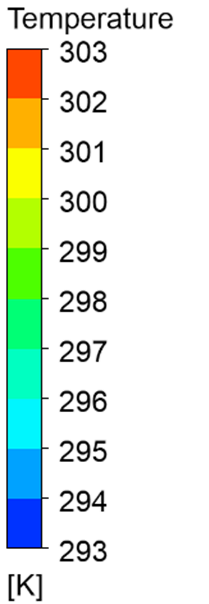
\includegraphics[width=\linewidth]{media/image40.png}
            \end{minipage}
        } &
        \begin{minipage}[t]{0.17\textwidth}
            \centering
            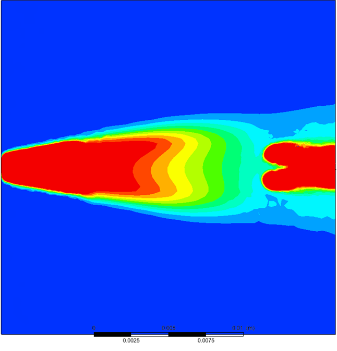
\includegraphics[width=\textwidth]{media/image41.png}\\
            \vspace{-1em}
            {\scriptsize\textbf{(a) $\theta_c$ = 12\degree}}
        \end{minipage} &
        \begin{minipage}[t]{0.17\textwidth}
            \centering
            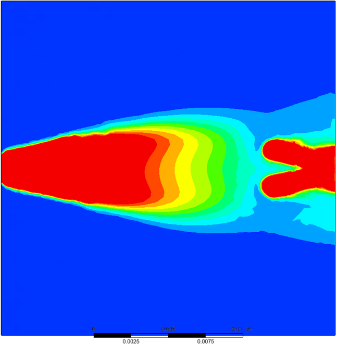
\includegraphics[width=\textwidth]{media/image43.png}\\
            \vspace{-1em}
            {\scriptsize\textbf{(b) $\theta_c$ = 17\degree}}
        \end{minipage} &
        \begin{minipage}[t]{0.17\textwidth}
            \centering
            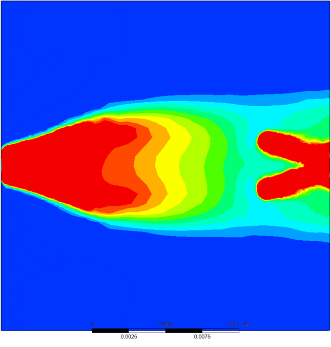
\includegraphics[width=\textwidth]{media/image44.png}\\
            \vspace{-1em}
            {\scriptsize\textbf{(c) $\theta_c$ = 22\degree}}
        \end{minipage} &
        \begin{minipage}[t]{0.17\textwidth}
            \centering
            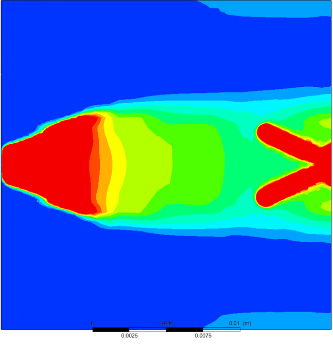
\includegraphics[width=\textwidth]{media/image45.png}\\
            \vspace{-1em}
            {\scriptsize\textbf{(d) $\theta_c$ = 27\degree}}
        \end{minipage} \\
         &\begin{minipage}[t]{0.17\textwidth}
            \centering
            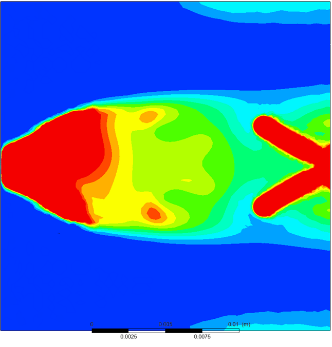
\includegraphics[width=\textwidth]{media/image46.png}\\
            \vspace{-1em}
            {\scriptsize\textbf{(e) $\theta_c$ = 32\degree}}
        \end{minipage} &
        \begin{minipage}[t]{0.17\textwidth}
            \centering
            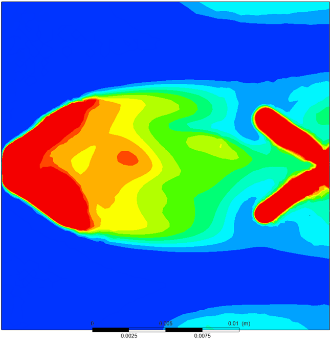
\includegraphics[width=\textwidth]{media/image47.png}\\
            \vspace{-1em}
            {\scriptsize\textbf{(f) $\theta_c$ = 37\degree}}
        \end{minipage} &
        \begin{minipage}[t]{0.17\textwidth}
            \centering
            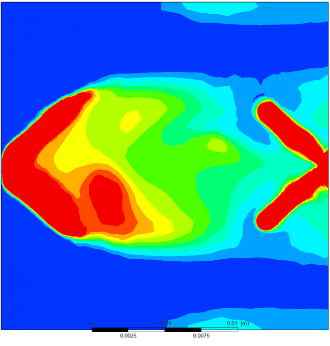
\includegraphics[width=\textwidth]{media/image48.png}\\
            \vspace{-1em}
            {\scriptsize\textbf{(g) $\theta_c$ = 42\degree}}
        \end{minipage} & \\
    \end{tabular}
    \caption{Temperature distribution of middle $z$-axis section of CPHE with various $\theta_c$.}
    \label{figure11}
\end{figure}

From Fig.~\ref{figure11}, it is shown that the higher temperature, which indicates the better heat transfer, is more concentrated in the middle $y$-axis plane for lower $\theta_c$. When $\theta_c$ increases, the temperature profile expands from the middle $y$-axis towards the two ends. Smaller hot spots and higher temperatures around and behind the concave capsules are found in higher $\theta_c$ (Fig.~\ref{figure11}(e), (f), and (g)). As discussed above, it is due to the reduced recirculating flow in the middle of the computational domain caused by the redirection of the convex capsules, and introducing more small eddies along the middle $x$-axis that causes better mixing of fluid. The turbulence along the middle $x$-axis will also force more mixing within the concave capsule region, which further enhances the heat transfer.

\subsubsection{Capsule height}
\label{sec:capsule_height_results}

Other than the capsule angle $\theta_c$, the height of the capsule $C_h$ would also alter the cross-section of the fluid domain, which will affect the pressure drop and heat transfer of CPHE. For this study, $C_h$ ranging from 2~mm to 5~mm with 0.5~mm increments was studied to investigate the effect of different capsule heights on the performance of CPHE.

\begin{figure}[H]
    \centering
    \renewcommand{\arraystretch}{1.0}
    \begin{tabular}{ccccc}
        \multirow{2}{*}{
            \begin{minipage}[c]{0.14\textwidth}
                \centering
                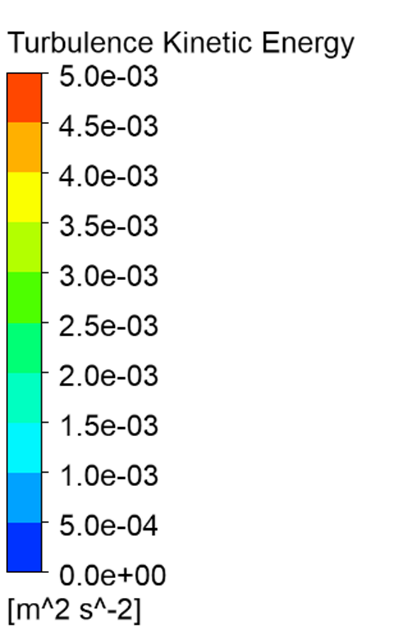
\includegraphics[width=\linewidth]{media/image50.png}
            \end{minipage}
        } &
        \begin{minipage}[t]{0.17\textwidth}
            \centering
            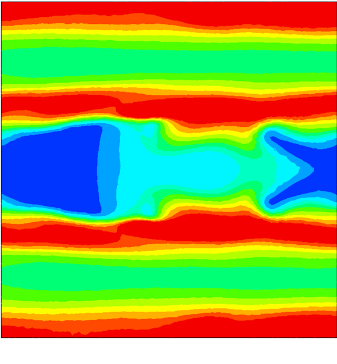
\includegraphics[width=\textwidth]{media/image49.png}\\
            \vspace{-1em}
            {\scriptsize\textbf{(a) $C_h/l_c$ = 0.09}}
        \end{minipage} &
        \begin{minipage}[t]{0.17\textwidth}
            \centering
            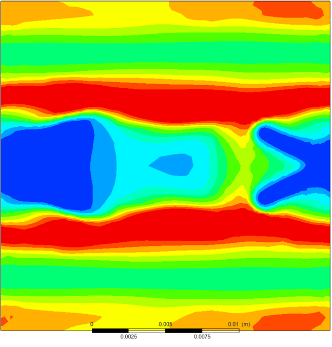
\includegraphics[width=\textwidth]{media/image21.png}\\
            \vspace{-1em}
            {\scriptsize\textbf{(b) $C_h/l_c$ = 0.11}}
        \end{minipage} &
        \begin{minipage}[t]{0.17\textwidth}
            \centering
            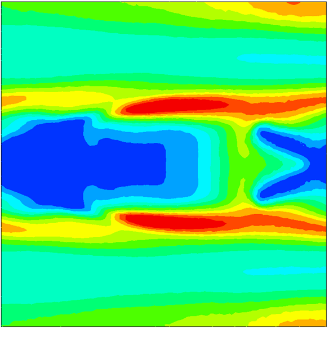
\includegraphics[width=\textwidth]{media/image52.png}\\
            \vspace{-1em}
            {\scriptsize\textbf{(c) $C_h/l_c$ = 0.13}}
        \end{minipage} &
        \begin{minipage}[t]{0.17\textwidth}
            \centering
            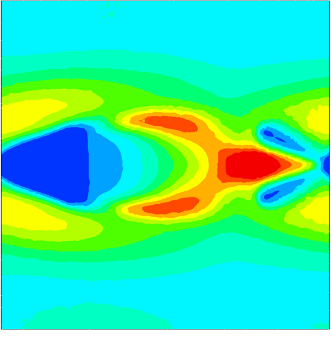
\includegraphics[width=\textwidth]{media/image53.png}\\
            \vspace{-1em}
            {\scriptsize\textbf{(d) $C_h/l_c$ = 0.16}}
        \end{minipage} \\
        & \begin{minipage}[t]{0.17\textwidth}
            \centering
            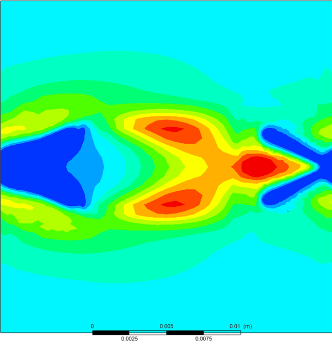
\includegraphics[width=\textwidth]{media/image54.png}\\
            \vspace{-1em}
            {\scriptsize\textbf{(e) $C_h/l_c$ = 0.18}}
        \end{minipage} &
        \begin{minipage}[t]{0.17\textwidth}
            \centering
            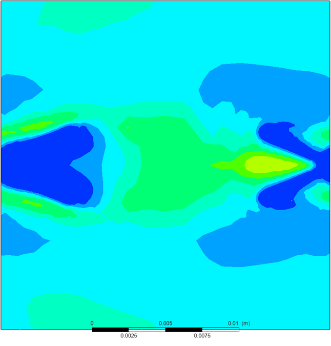
\includegraphics[width=\textwidth]{media/image55.png}\\
            \vspace{-1em}
            {\scriptsize\textbf{(f) $C_h/l_c$ = 0.2}}
        \end{minipage} &
        \begin{minipage}[t]{0.17\textwidth}
            \centering
            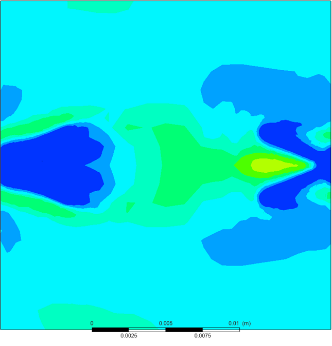
\includegraphics[width=\textwidth]{media/image56.png}\\
            \vspace{-1em}
            {\scriptsize\textbf{(g) $C_h/l_c$ = 0.22}}
        \end{minipage} & \\
    \end{tabular}
    \caption{TKE distribution of middle $z$-axis section of CPHE with various $C_h/l_c$.}
    \label{figure12}
\end{figure}

\begin{figure}[H]
    \centering
    \renewcommand{\arraystretch}{1.1}
    \begin{tabular}{cccc}
        \begin{minipage}[t]{0.2\textwidth}
            \centering
            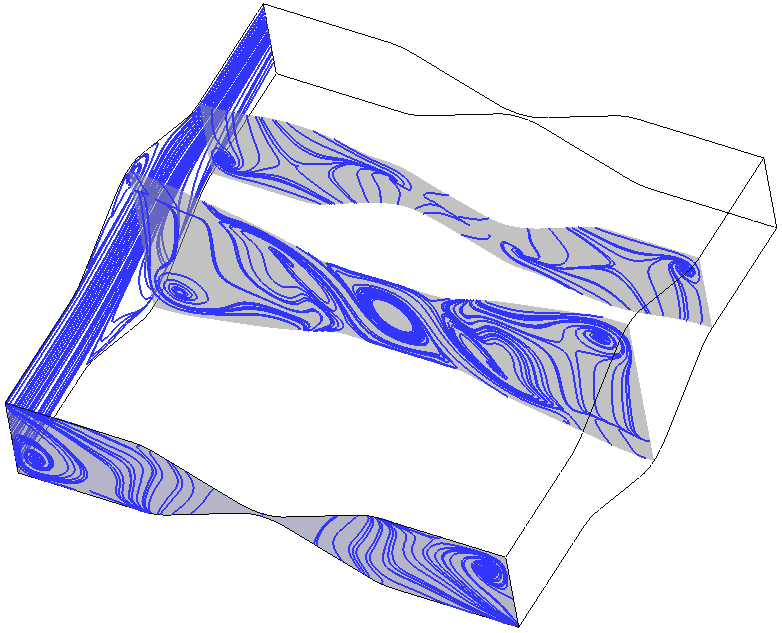
\includegraphics[width=\textwidth]{media/2D_stream_CH_2.png}
            {\scriptsize\textbf{(a) $C_h/l_c$ = 0.09}}
        \end{minipage} &
        \begin{minipage}[t]{0.21\textwidth}
            \centering
            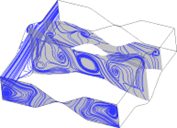
\includegraphics[width=\textwidth]{media/Picture1.png}
            {\scriptsize\textbf{(b) $C_h/l_c$ = 0.11}}
        \end{minipage} &
        \begin{minipage}[t]{0.2\textwidth}
            \centering
            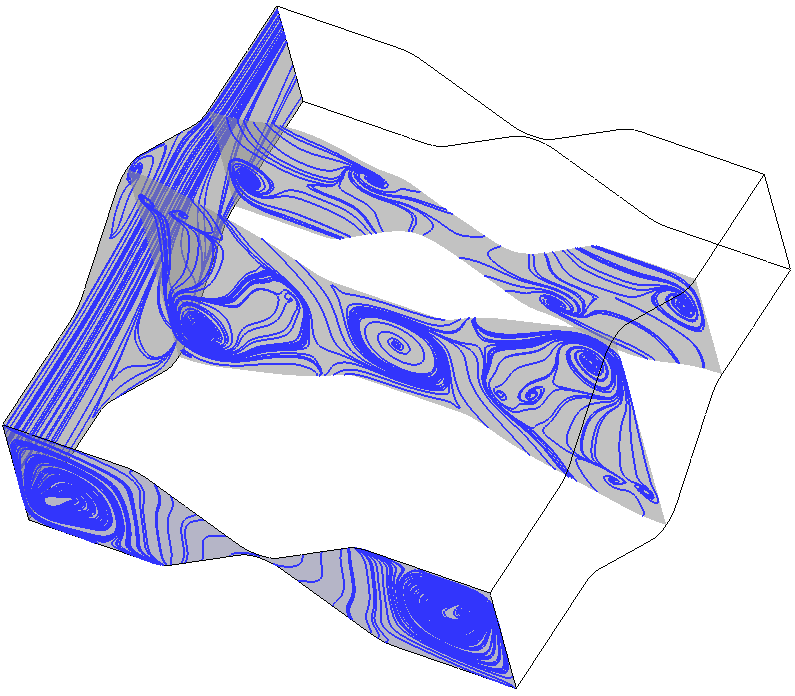
\includegraphics[width=\textwidth]{media/2D_stream_CH_3.png}
            {\scriptsize\textbf{(c) $C_h/l_c$ = 0.13}}
        \end{minipage} &
        \begin{minipage}[t]{0.2\textwidth}
            \centering
            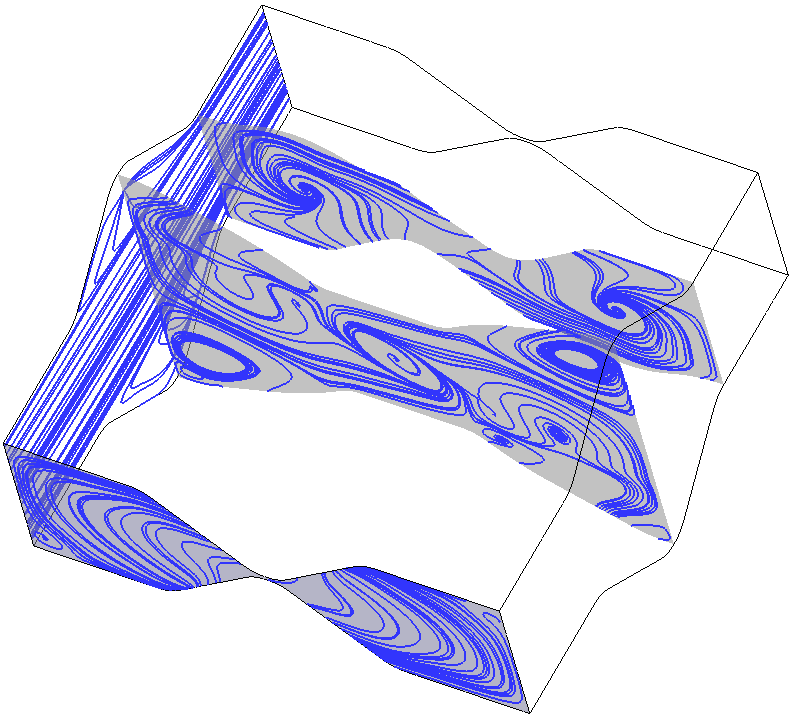
\includegraphics[width=\textwidth]{media/2D_stream_CH_3_5.png}
            {\scriptsize\textbf{(d) $C_h/l_c$ = 0.16}}
        \end{minipage} \\
        \begin{minipage}[t]{0.2\textwidth}
            \centering
            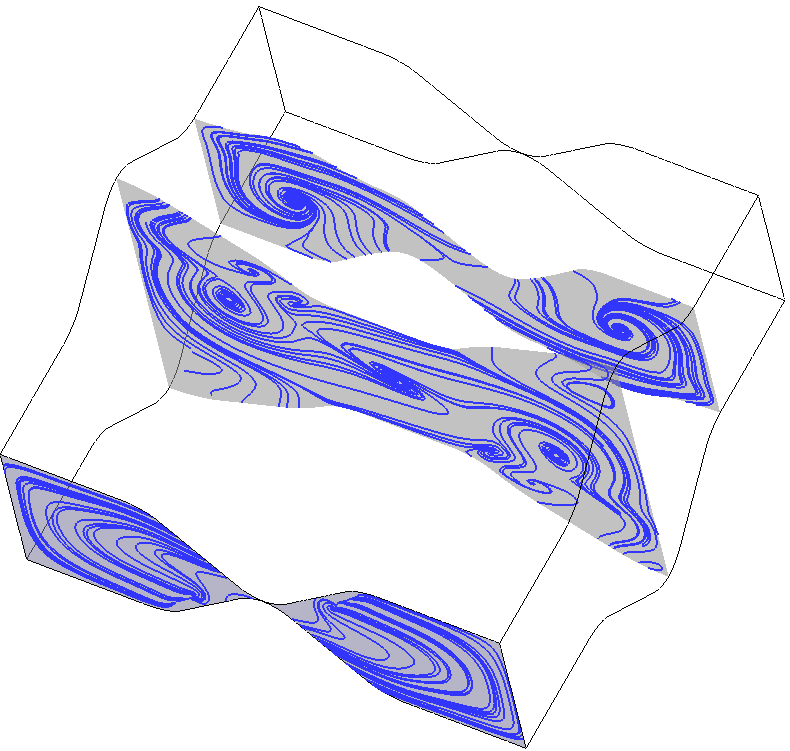
\includegraphics[width=\textwidth]{media/2D_stream_CH_4.png}
            {\scriptsize\textbf{(e) $C_h/l_c$ = 0.18}}
        \end{minipage} &
        \begin{minipage}[t]{0.2\textwidth}
            \centering
            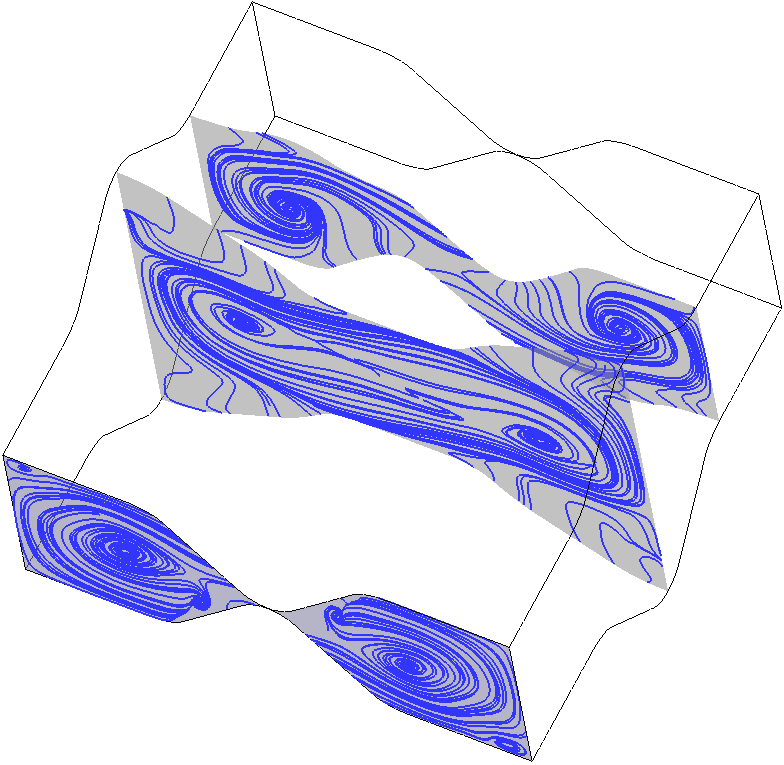
\includegraphics[width=\textwidth]{media/2D_stream_CH_4_5.png}
            {\scriptsize\textbf{(f) $C_h/l_c$ = 0.2}}
        \end{minipage} &
    \begin{minipage}[t]{0.2\textwidth}
        \centering
        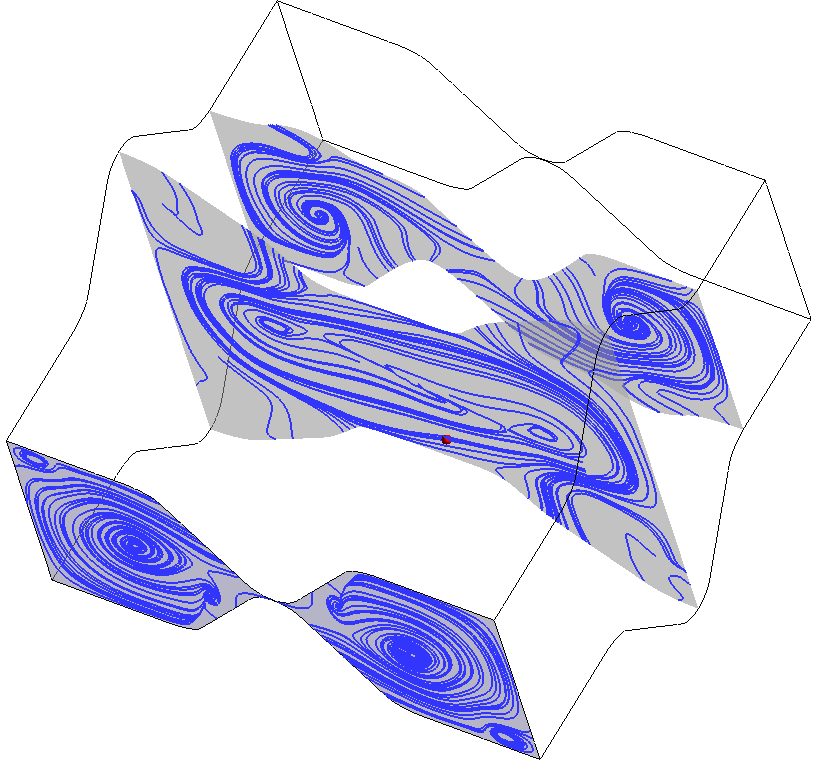
\includegraphics[width=\textwidth]{media/2D_stream_CH_5.png}
        {\scriptsize\textbf{(g) $C_h/l_c$ = 0.22}}
    \end{minipage} &
     \begin{minipage}[t]{0.2\textwidth}
            \centering
            
\includegraphics[width=\textwidth]{media/Screenshot_2025-08-01_205019.png}
    \end{minipage} \\
    \end{tabular}
    \caption{2D streamlines of CPHE with various $C_h/l_c$.}
    \label{figure13}
\end{figure}

It is observed that the TKE is diminishing when the height of the capsule increases. Despite the magnitude, the distribution of TKE changes from higher TKE channels along the stream-wise direction (Fig.~\ref{figure12}(a)) to more center concentrated (Fig.~\ref{figure12}(e)). Increasing $C_h$ enlarges the channel cross-sectional area, which has two related but distinct effects: (a) the global mean velocity decreases because the same mass flow rate passes through a larger cross-section, and (b) locally, the flow accelerates less sharply as it passes over the convex capsule features, weakening the shear layers that would otherwise generate small-scale eddies (Fig.~\ref{figure13}(a) vs Fig.~\ref{figure13}(e)). The net result is that fewer but larger and more uniform eddies are produced, which regulate the flow field and encourage mixing between different flow regions. Similar to increasing $\theta_c$, increasing $C_h$ also reduces the wake region behind convex capsules, due to the increased cross-sectional area, which reduces the effect of the shape of convex capsules on redirecting the flow towards the two ends of the spanwise direction. The increased volume in the concave region also helps reduce the mean velocity and causes more recirculating flows.

\begin{figure}[H]
    \centering
    \renewcommand{\arraystretch}{1.1}
    \begin{tabular}{ccccc}
    \multirow{2}{*}{
   \begin{minipage}[c]{0.09\textwidth} 
    \centering
    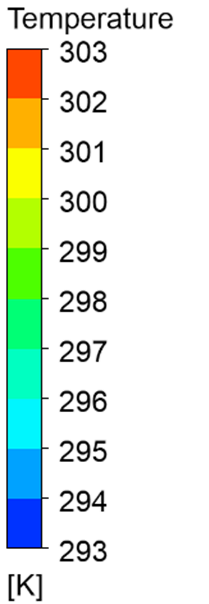
\includegraphics[width=\linewidth]{media/image40.png}
  \end{minipage}
} & 
        \begin{minipage}[t]{0.17\textwidth}
            \centering
            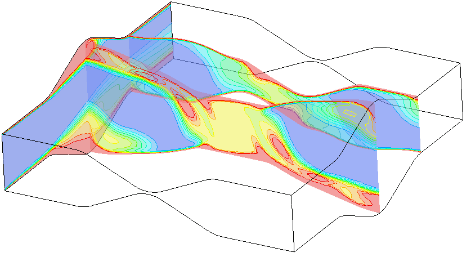
\includegraphics[width=\textwidth]{media/image69.png}
            {\scriptsize\textbf{(a) $C_h/l_c$ = 0.09}}
        \end{minipage} &
        \begin{minipage}[t]{0.17\textwidth}
            \centering
            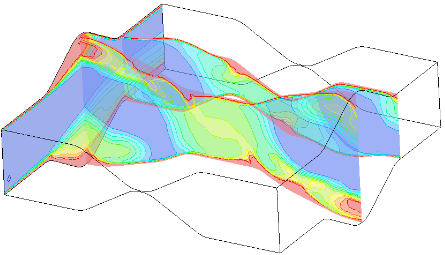
\includegraphics[width=\textwidth]{media/image70.png}
            {\scriptsize\textbf{(b) $C_h/l_c$ = 0.11}}
        \end{minipage} &
        \begin{minipage}[t]{0.17\textwidth}
            \centering
            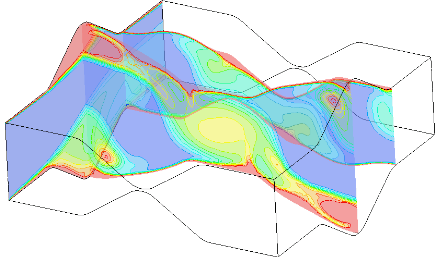
\includegraphics[width=\textwidth]{media/image71.png}
            {\scriptsize\textbf{(c) $C_h/l_c$ = 0.13}}
        \end{minipage} &
        \begin{minipage}[t]{0.17\textwidth}
            \centering
            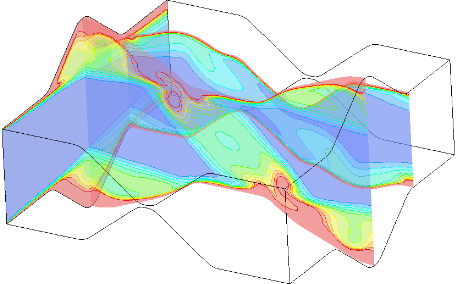
\includegraphics[width=\textwidth]{media/image72.png}
            {\scriptsize\textbf{(d) $C_h/l_c$ = 0.16}}
        \end{minipage} \\ &
        \begin{minipage}[t]{0.17\textwidth}
            \centering
            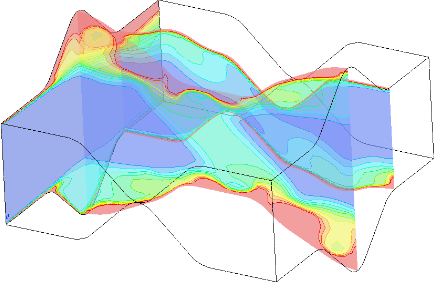
\includegraphics[width=\textwidth]{media/image73.png}
            {\scriptsize\textbf{(e) $C_h/l_c$ = 0.18}}
        \end{minipage} &
        \begin{minipage}[t]{0.17\textwidth}
            \centering
            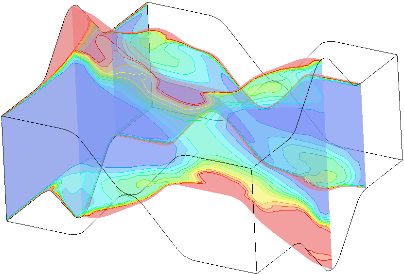
\includegraphics[width=\textwidth]{media/image74.png}
            {\scriptsize\textbf{(f) $C_h/l_c$ = 0.2}}
        \end{minipage} &
    \begin{minipage}[t]{0.17\textwidth}
        \centering
        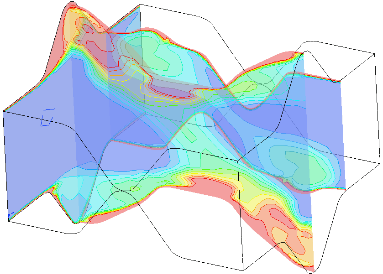
\includegraphics[width=\textwidth]{media/image75.png}
        {\scriptsize\textbf{(g) $C_h/l_c$ = 0.22}}
    \end{minipage} &
    \begin{minipage}[t]{0.17\textwidth}
        \centering
        
\includegraphics[width=\textwidth]{media/Screenshot_2025-08-01_205019.png} 
    \end{minipage} \\
    \end{tabular}
    \caption{Temperature distribution of CPHE with various $C_h/l_c$.}
    \label{figure15}
\end{figure}

For lower capsule height, as the mean velocity along the side of convex capsules is high, the majority of convective heat transfer takes place in the center of the unit cell, which is due to the wake region generated by the convex capsules, causing more recirculating flows and enhancing the heat transfer locally (Fig.~\ref{figure15}(a)). When the capsule height increases, the major heat transfer location is transferred to the concave regions, where the recirculating flows take place (Fig.~\ref{figure15}(f) \& (g)), and as mentioned above, the center mixing region is less effective for higher capsule heights.

\clearpage

\subsection{DPHE parametric study}
\label{sec:dphe_results}

Dimple pattern has also been investigated in this study. To benchmark the performance of DPHE, two main parameters are investigated in this study to explore their impact on the pressure drop and heat transfer rate: 1) dimple height; 2) dimple spacing.

\subsubsection{Dimple height}
\label{sec:dimple_height_results}

As the study of capsule height shows a positive relationship between Nusselt number and capsule height, the height of the dimple $D_h$ would also be studied to illustrate the performance of various embossing heights.

\begin{figure}[H]
    \centering
    \renewcommand{\arraystretch}{1.0}
    \begin{tabular}{ccccc}
        \multirow{2}{*}{
            \begin{minipage}[c]{0.14\textwidth}
                \centering
                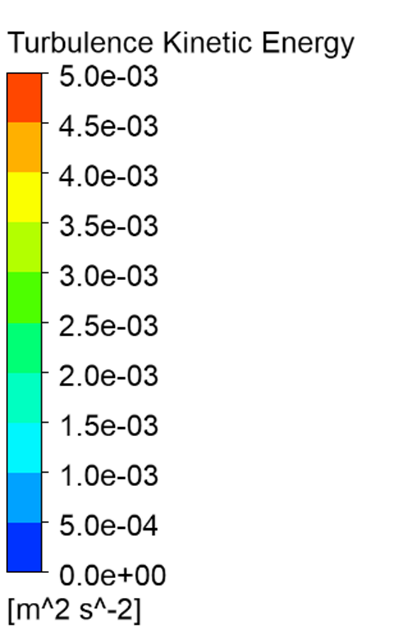
\includegraphics[width=\linewidth]{media/image50.png}
            \end{minipage}
        } &
        \begin{minipage}[t]{0.18\textwidth}
            \centering
            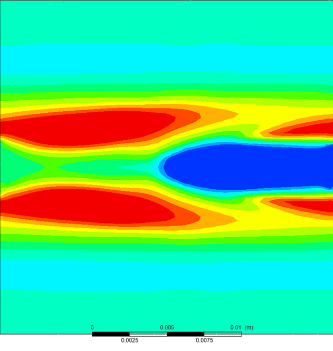
\includegraphics[width=\textwidth]{media/image76.png}\\
            \vspace{-1em}
            {\scriptsize\textbf{(a) $D_h/l_d$ = 0.09}}
        \end{minipage} &
        \begin{minipage}[t]{0.18\textwidth}
            \centering
            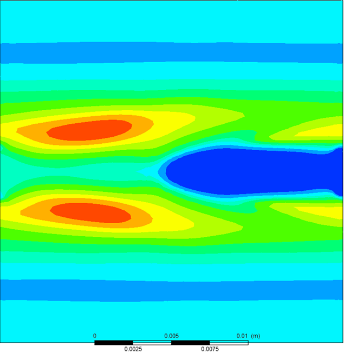
\includegraphics[width=\textwidth]{media/image77.png}\\
            \vspace{-1em}
            {\scriptsize\textbf{(b) $D_h/l_d$ = 0.11}}
        \end{minipage} &
        \begin{minipage}[t]{0.18\textwidth}
            \centering
            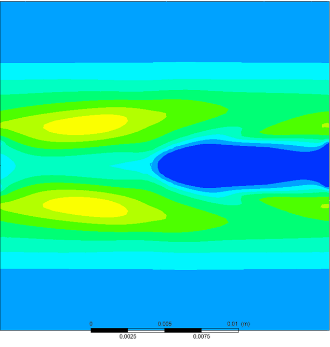
\includegraphics[width=\textwidth]{media/image78.png}\\
            \vspace{-1em}
            {\scriptsize\textbf{(c) $D_h/l_d$ = 0.13}}
        \end{minipage} &
        \begin{minipage}[t]{0.18\textwidth}
            \centering
            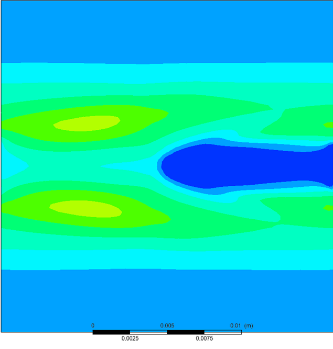
\includegraphics[width=\textwidth]{media/image79.png}\\
            \vspace{-1em}
            {\scriptsize\textbf{(d) $D_h/l_d$ = 0.16}}
        \end{minipage} \\
        & \begin{minipage}[t]{0.18\textwidth}
            \centering
            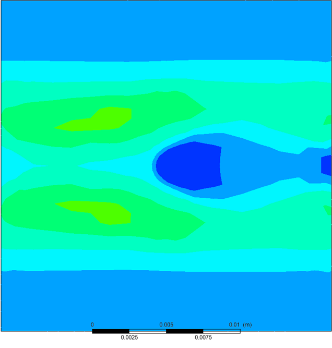
\includegraphics[width=\textwidth]{media/image80.png}\\
            \vspace{-1em}
            {\scriptsize\textbf{(e) $D_h/l_d$ = 0.18}}
        \end{minipage} &
        \begin{minipage}[t]{0.18\textwidth}
            \centering
            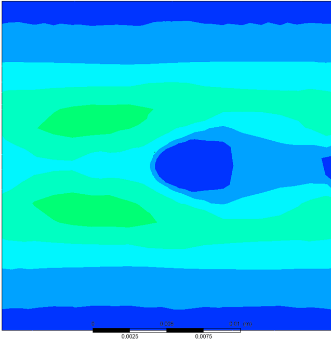
\includegraphics[width=\textwidth]{media/image81.png}\\
            \vspace{-1em}
            {\scriptsize\textbf{(f) $D_h/l_d$ = 0.2}}
        \end{minipage} &
        \begin{minipage}[t]{0.18\textwidth}
            \centering
            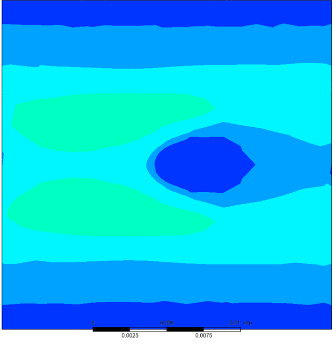
\includegraphics[width=\textwidth]{media/image82.png}\\
            \vspace{-1em}
            {\scriptsize\textbf{(g) $D_h/l_d$ = 0.22}}
        \end{minipage} & \\
    \end{tabular}
    \caption{TKE distribution of middle $z$-axis section of DPHE with various $D_h/l_d$.}
    \label{figure16}
\end{figure}

\begin{figure}[H]
    \centering
    \renewcommand{\arraystretch}{1.1}
    \begin{tabular}{cccc}
        \begin{minipage}[t]{0.2\textwidth}
            \centering
            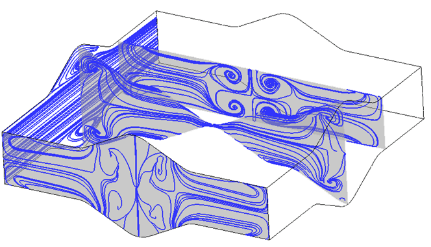
\includegraphics[width=\textwidth]{media/image83.png}
            {\scriptsize\textbf{(a) $D_h/l_d$ = 0.09}}
        \end{minipage} &
        \begin{minipage}[t]{0.2\textwidth}
            \centering
            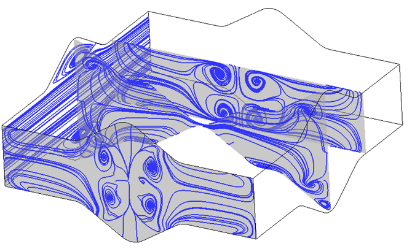
\includegraphics[width=\textwidth]{media/image84.png}
            {\scriptsize\textbf{(b) $D_h/l_d$ = 0.11}}
        \end{minipage} &
        \begin{minipage}[t]{0.2\textwidth}
            \centering
            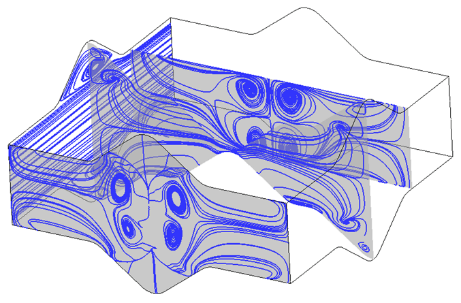
\includegraphics[width=\textwidth]{media/image85.png}
            {\scriptsize\textbf{(c) $D_h/l_d$ = 0.13}}
        \end{minipage} &
        \begin{minipage}[t]{0.2\textwidth}
            \centering
            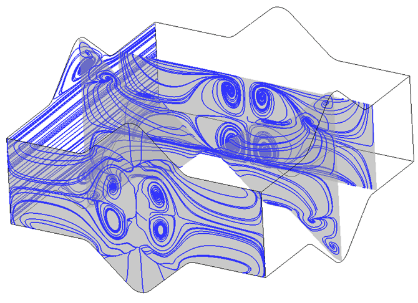
\includegraphics[width=\textwidth]{media/image86.png}
            {\scriptsize\textbf{(d) $D_h/l_d$ = 0.16}}
        \end{minipage} \\
        \begin{minipage}[t]{0.2\textwidth}
            \centering
            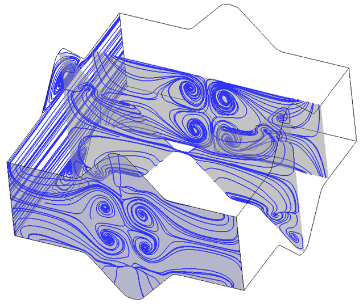
\includegraphics[width=\textwidth]{media/image87.png}
            {\scriptsize\textbf{(e) $D_h/l_d$ = 0.18}}
        \end{minipage} &
        \begin{minipage}[t]{0.2\textwidth}
            \centering
            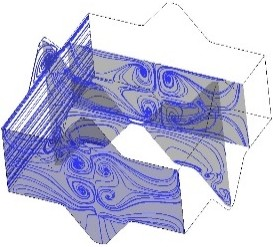
\includegraphics[width=\textwidth]{media/image88.jpeg}
            {\scriptsize\textbf{(f) $D_h/l_d$ = 0.2}}
        \end{minipage} &
    \begin{minipage}[t]{0.2\textwidth}
        \centering
        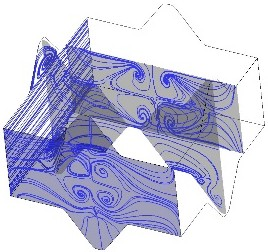
\includegraphics[width=\textwidth]{media/image89.jpeg}
        {\scriptsize\textbf{(g) $D_h/l_d$ = 0.22}}
    \end{minipage} &
     \begin{minipage}[t]{0.2\textwidth}
            \centering
            
\includegraphics[width=\textwidth]{media/Screenshot_2025-08-01_205019.png}
    \end{minipage} \\
    \end{tabular}
    \caption{2D streamlines of DPHE with various $D_h/l_d$.}
    \label{figure17}
\end{figure}

\begin{figure}[H]
    \centering
    \renewcommand{\arraystretch}{1.1}
    \begin{tabular}{ccccc}
    \multirow{2}{*}{
  \begin{minipage}[c]{0.10\textwidth}  
    \centering
    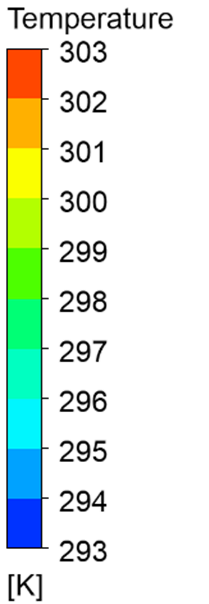
\includegraphics[width=\linewidth]{media/image40.png}
  \end{minipage}
} & 
        \begin{minipage}[t]{0.2\textwidth}
            \centering
            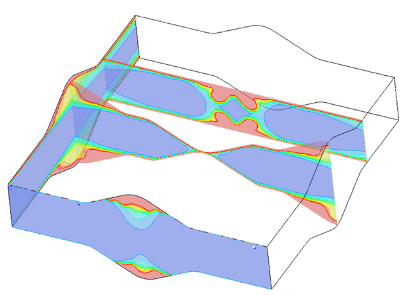
\includegraphics[width=\textwidth]{media/image90.png}
            {\scriptsize\textbf{(a) $D_h/l_d$ = 0.09}}
        \end{minipage} &
        \begin{minipage}[t]{0.2\textwidth}
            \centering
            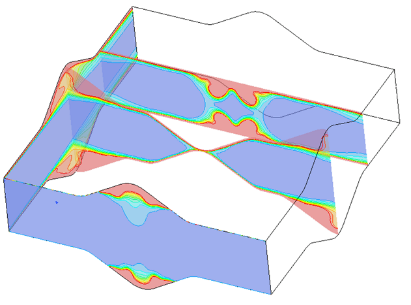
\includegraphics[width=\textwidth]{media/image91.png}
            {\scriptsize\textbf{(b) $D_h/l_d$ = 0.11}}
        \end{minipage} &
        \begin{minipage}[t]{0.2\textwidth}
            \centering
            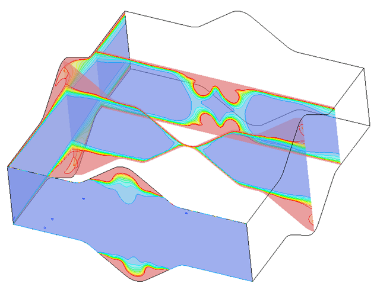
\includegraphics[width=\textwidth]{media/image92.png}
            {\scriptsize\textbf{(c) $D_h/l_d$ = 0.13}}
        \end{minipage} &
        \begin{minipage}[t]{0.2\textwidth}
            \centering
            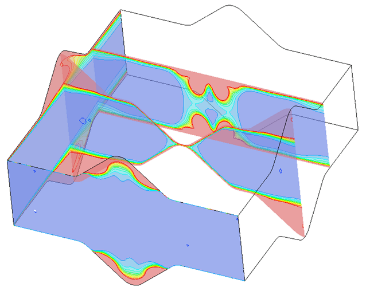
\includegraphics[width=\textwidth]{media/image93.png}
            {\scriptsize\textbf{(d) $D_h/l_d$ = 0.16}}
        \end{minipage} \\ &
        \begin{minipage}[t]{0.2\textwidth}
            \centering
            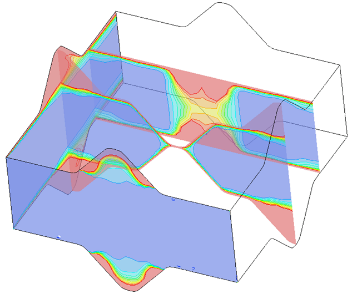
\includegraphics[width=\textwidth]{media/image94.png}
            {\scriptsize\textbf{(e) $D_h/l_d$ = 0.18}}
        \end{minipage} &
        \begin{minipage}[t]{0.2\textwidth}
            \centering
            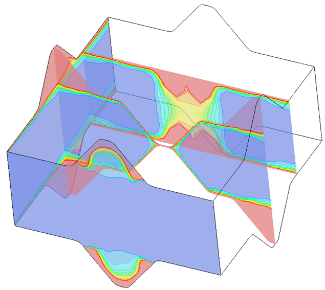
\includegraphics[width=\textwidth]{media/image95.png}
            {\scriptsize\textbf{(f) $D_h/l_d$ = 0.2}}
        \end{minipage} &
    \begin{minipage}[t]{0.2\textwidth}
        \centering
        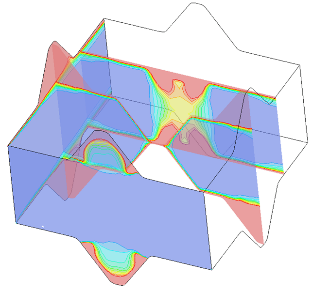
\includegraphics[width=\textwidth]{media/image96.png}
        {\scriptsize\textbf{(g) $D_h/l_d$ = 0.22}}
    \end{minipage} &
    \begin{minipage}[t]{0.2\textwidth}
        \centering
        
\includegraphics[width=\textwidth]{media/Screenshot_2025-08-01_205019.png} 
    \end{minipage} \\
    \end{tabular}
    \caption{3D temperature distribution of DPHE with various $D_h/l_d$.}
    \label{figure18}
\end{figure}

Smaller dimple heights concentrate TKE along the side of the convex dimple, creating distinct wake regions behind the convex dimple (Fig.~\ref{figure16}(a)). This concentration of TKE enhances fluid mixing and generates strong, localized vortices, which improve the overall flow dynamics. The wake region causes certain recirculating flows. Conversely, larger dimple heights reduce average TKE levels due to the dampening effect of the larger volume, which disrupts the wake zone behind the convex dimple. The increased volume tends to draw fluid flows towards the concave region, which generates a large portion of recirculating flow among those regions.

Lower dimple heights enhance heat transfer locally by generating strong, localized vortices that increase the local heat transfer coefficients. The changes in direction and flow separation around the convex dimples lead to less effective convective heat transfer due to ineffective mixing of fluid layers near the heat transfer surfaces (Fig.~\ref{figure18}(a)). Due to the larger volume in the middle $x$-axis, the mean velocity of the flow reduces, and this reduces the wake zone generated by the convex dimple. The reduced wake zone disrupts the vortices at the side of the convex dimple and improves the mixing of fluid layers (Fig.~\ref{figure18}(a) vs Fig.~\ref{figure18}(e)).

\subsubsection{Dimple spacing}
\label{sec:dimple_spacing_results}

In addition to height, angle, and shape, the arrangement of patterns significantly impacts performance \citep{jiang2019a, hamedi2024}. Although circular dimples lack a specific directional orientation, researching the spacing between dimples ($D_s$) could provide valuable insights for the research on fouling resistance, plate stability, and fluid-solid mix heat transfer medium.

\begin{figure}[H]
    \centering
    \renewcommand{\arraystretch}{1.1}
    \begin{tabular}{ccccc}
    \multirow{2}{*}{
  \begin{minipage}[c]{0.20\textwidth}  
    \centering
    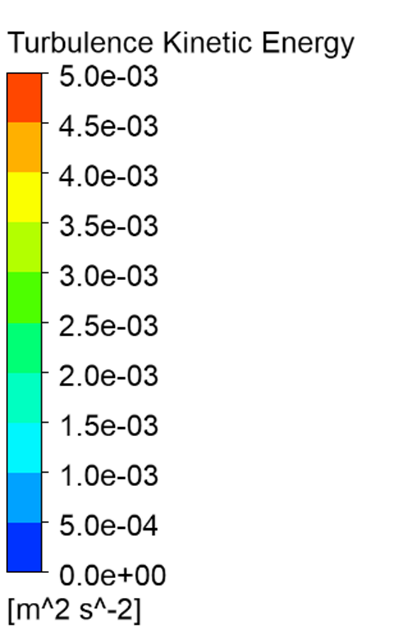
\includegraphics[width=\linewidth]{media/image50.png}
  \end{minipage}
} &
        \begin{minipage}[t]{0.18\textwidth}
            \centering
            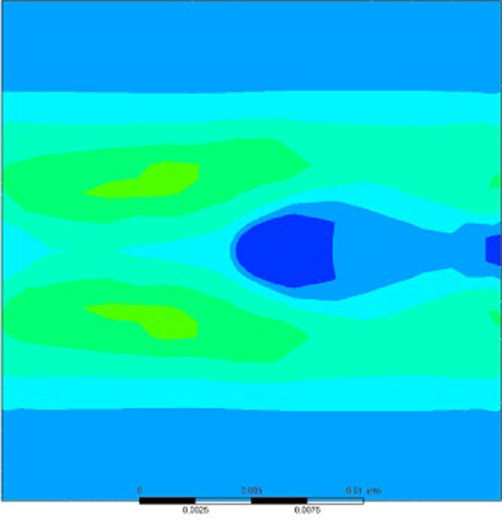
\includegraphics[width=\textwidth]{media/Picture5.png}\\
            \vspace{-1em}
            {\scriptsize\textbf{(a) $D_s/l_d$ = 0.05}}
        \end{minipage} &
        \begin{minipage}[t]{0.18\textwidth}
            \centering
            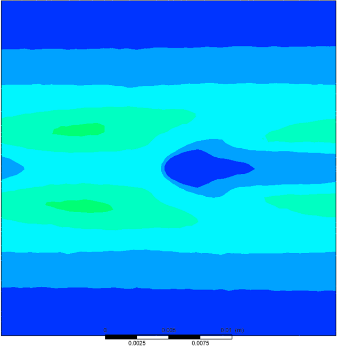
\includegraphics[width=\textwidth]{media/image97.png}\\
            \vspace{-1em}
            {\scriptsize\textbf{(b) $D_s/l_d$ = 0.14}}
        \end{minipage} &
        \begin{minipage}[t]{0.18\textwidth}
            \centering
            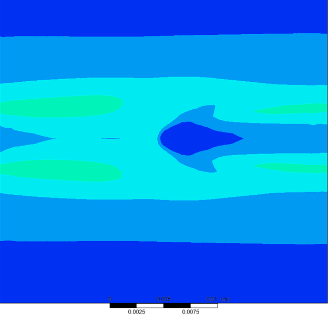
\includegraphics[width=\textwidth]{media/image98.png}\\
            \vspace{-1em}
            {\scriptsize\textbf{(c) $D_s/l_d$ = 0.23}}
        \end{minipage} \\ &
        \begin{minipage}[t]{0.18\textwidth}
            \centering
            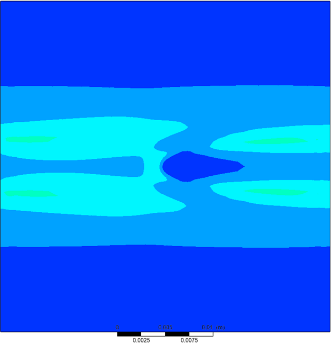
\includegraphics[width=\textwidth]{media/image99.png}\\
            \vspace{-1em}
            {\scriptsize\textbf{(d) $D_s/l_d$ = 0.32}}
        \end{minipage} &
        \begin{minipage}[t]{0.18\textwidth}
            \centering
            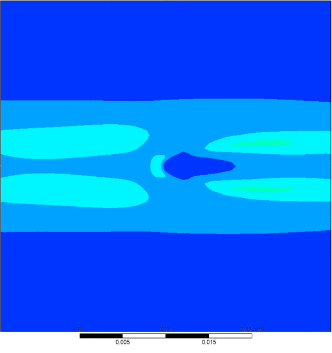
\includegraphics[width=\textwidth]{media/image100.png}\\
            \vspace{-1em}
            {\scriptsize\textbf{(e) $D_s/l_d$ = 0.41}}
        \end{minipage} &
        \begin{minipage}[t]{0.18\textwidth}
            \centering
            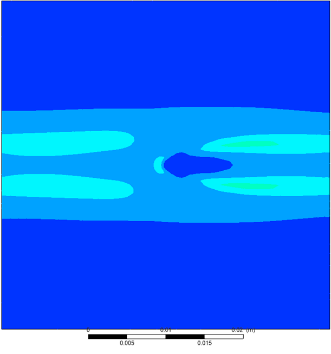
\includegraphics[width=\textwidth]{media/image101.png}\\
            \vspace{-1em}
            {\scriptsize\textbf{(f) $D_s/l_d$ = 0.5}}
        \end{minipage} \\
    \end{tabular}
    \caption{TKE distribution of middle $z$-axis section of DPHE with various $D_s/l_d$.}
    \label{figure19}
\end{figure}

\begin{figure}[H]
    \centering
    \renewcommand{\arraystretch}{1.1}
    \begin{tabular}{ccc}
        \begin{minipage}[t]{0.2\textwidth}
            \centering
            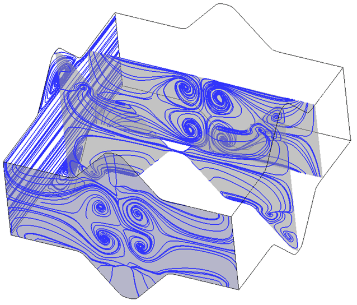
\includegraphics[width=\textwidth]{media/image102.png}
            {\scriptsize\textbf{(a) $D_s/l_d$ = 0.05}}
        \end{minipage} &
        \begin{minipage}[t]{0.225\textwidth}
            \centering
            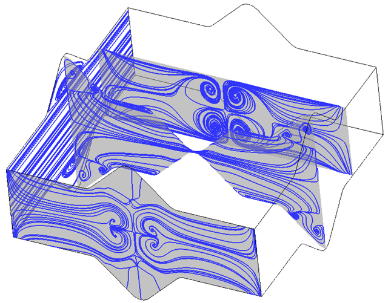
\includegraphics[width=\textwidth]{media/image103.png}
            {\scriptsize\textbf{(b) $D_s/l_d$ = 0.14}}
        \end{minipage} &
        \begin{minipage}[t]{0.225\textwidth}
            \centering
            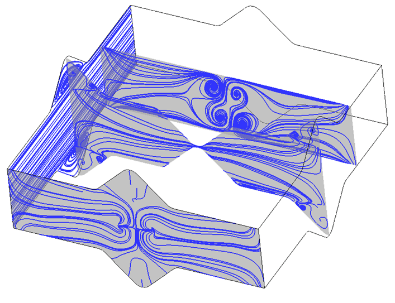
\includegraphics[width=\textwidth]{media/image104.png}
            {\scriptsize\textbf{(c) $D_s/l_d$ = 0.23}}
        \end{minipage} \\
        \begin{minipage}[t]{0.225\textwidth}
            \centering
            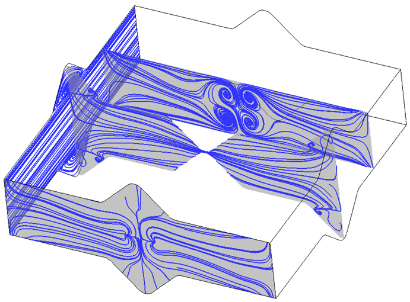
\includegraphics[width=\textwidth]{media/image105.png}
            {\scriptsize\textbf{(d) $D_s/l_d$ = 0.32}}
        \end{minipage} &
        \begin{minipage}[t]{0.225\textwidth}
            \centering
            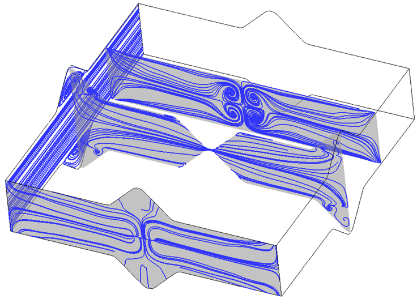
\includegraphics[width=\textwidth]{media/image106.png}
            {\scriptsize\textbf{(e) $D_s/l_d$ = 0.41}}
        \end{minipage} &
        \begin{minipage}[t]{0.225\textwidth}
            \centering
            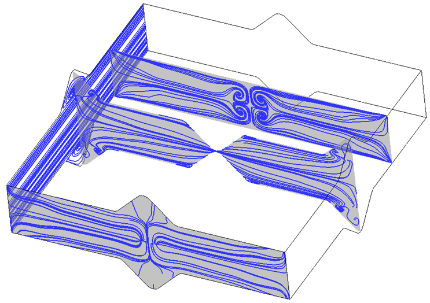
\includegraphics[width=\textwidth]{media/image107.png}
            {\scriptsize\textbf{(f) $D_s/l_d$ = 0.5}}
        \end{minipage} \\
    \end{tabular}
    \caption{2D streamlines of DPHE with various $D_s/l_d$.}
    \label{figure20}
\end{figure}

Wider dimple spacing isolates flow disturbances, reducing the development of turbulent regions and overall turbulence levels. This isolation results in fewer interactions between each iteration, leading to a more stable flow. With reduced turbulence, the fluid encounters less resistance, allowing for easier movement through the heat exchanger. In contrast, closely spaced dimples cause the wake regions behind each dimple to merge, intensifying turbulence and creating a more chaotic flow environment, which can be identified from the inlet of the unit cell (Fig.~\ref{figure21}(a) and (f)). This increased turbulence leads to higher resistance to fluid movement and more vigorous mixing of fluid layers. The merging of wake regions enhances vortex formation and interaction, contributing to a more complex and energetically dynamic flow field.

\begin{figure}[H]
    \centering
    \renewcommand{\arraystretch}{1.1}
    \begin{tabular}{ccccc}
  \multirow{2}{*}{
  \begin{minipage}[c]{0.10\textwidth}  
    \centering
    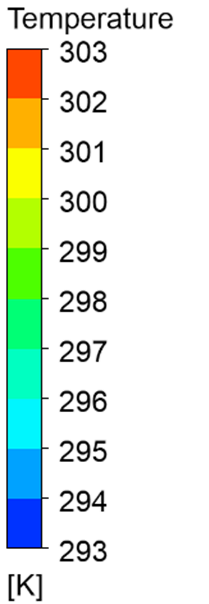
\includegraphics[width=\linewidth]{media/image40.png}
  \end{minipage}
} & 
        \begin{minipage}[t]{0.18\textwidth}
            \centering
            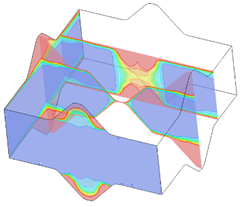
\includegraphics[width=\textwidth]{media/image108.png}
            {\scriptsize\textbf{(a) $D_s/l_d$ = 0.05}}
        \end{minipage} &
        \begin{minipage}[t]{0.18\textwidth}
            \centering
            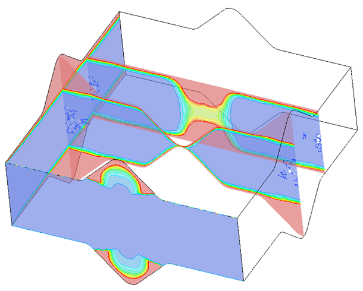
\includegraphics[width=\textwidth]{media/image109.png}
            {\scriptsize\textbf{(b) $D_s/l_d$ = 0.14}}
        \end{minipage} &
        \begin{minipage}[t]{0.18\textwidth}
            \centering
            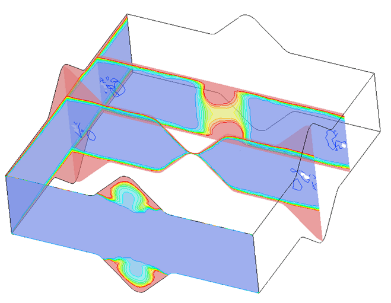
\includegraphics[width=\textwidth]{media/image110.png}
            {\scriptsize\textbf{(c) $D_s/l_d$ = 0.23}}
        \end{minipage} \\ &
        \begin{minipage}[t]{0.18\textwidth}
            \centering
            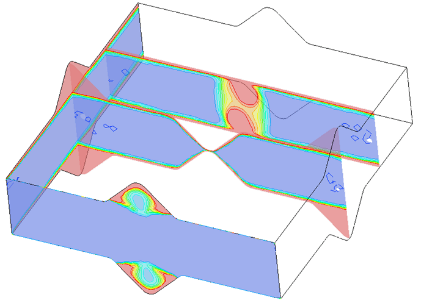
\includegraphics[width=\textwidth]{media/image111.png}
            {\scriptsize\textbf{(d) $D_s/l_d$ = 0.32}}
        \end{minipage} &
        \begin{minipage}[t]{0.18\textwidth}
            \centering
            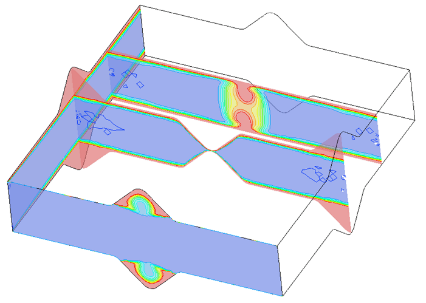
\includegraphics[width=\textwidth]{media/image112.png}
            {\scriptsize\textbf{(e) $D_s/l_d$ = 0.41}}
        \end{minipage} &
        \begin{minipage}[t]{0.18\textwidth}
            \centering
            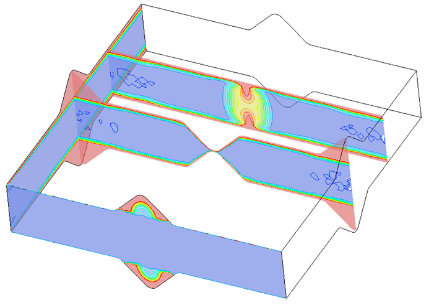
\includegraphics[width=\textwidth]{media/image113.png}
            {\scriptsize\textbf{(f) $D_s/l_d$ = 0.5}}
        \end{minipage} \\
    \end{tabular}
    \caption{3D temperature distribution of DPHE with various $D_s/l_d$.}
    \label{figure21}
\end{figure}

In terms of heat transfer, wider dimple spacing leads to less effective fluid mixing, which diminishes heat transfer performance as the spacing increases. The isolation of turbulent regions with wider spacing limits the interaction between hot and cold fluid zones, reducing the overall efficiency of heat exchange (Fig.~\ref{figure21}(f)). Conversely, closely spaced dimples promote enhanced vortex formation and interaction, significantly improving fluid mixing. This increased mixing facilitates more effective thermal energy transfer between the fluid and the heat exchanger surfaces, boosting heat transfer efficiency (Fig.~\ref{figure21}(a)). However, this improvement in heat transfer comes with the drawback of higher friction factors due to the intensified turbulence and chaotic flow conditions.


\section{Discussion}
\label{sec:discussion}

This section synthesizes the flow-physics observations presented in Section~\ref{sec:results} into quantitative friction-factor and Nusselt-number trends, reconciles the apparently contradictory behavior of $f$ and $\Delta p$ where it arises, and provides design recommendations for each parameter family.

\subsection{Capsule angle}
\label{sec:disc_capsule_angle}

As shown in Section~\ref{sec:capsule_angle_results}, increasing the capsule angle $\theta_c$ progressively disrupts the wake behind the convex capsules, introduces finer eddies, and shifts the dominant heat-transfer site towards the concave cavities. These flow-field changes manifest quantitatively as a monotonic increase in both friction factor and Nusselt number with $\theta_c$ (Fig.~\ref{figure22}). However, the friction penalty grows faster than the thermal gain: higher angles increase the extent of flow separation and boundary-layer disruption, so the pumping cost rises disproportionately.

Fig.~\ref{figure22} confirms that both Nu and $f$ increase monotonically with $\theta_c$, but the rise in $f$ is disproportionately large relative to the Nu gain, yielding diminishing thermo-hydraulic returns at wider capsule angles. For applications where energy efficiency and minimal pumping power are critical, lower angles (12\degree--17\degree) are therefore recommended, as they achieve modest Nu at a comparatively low friction penalty. Higher angles (37\degree--42\degree) are better suited for thermally demanding applications where maximizing heat transfer is the primary objective, despite the steep increase in $f$. Intermediate angles (22\degree--32\degree) provide a balanced compromise, making them suitable for general-purpose thermal-fluid systems.

\begin{figure}[H]
  \centering
  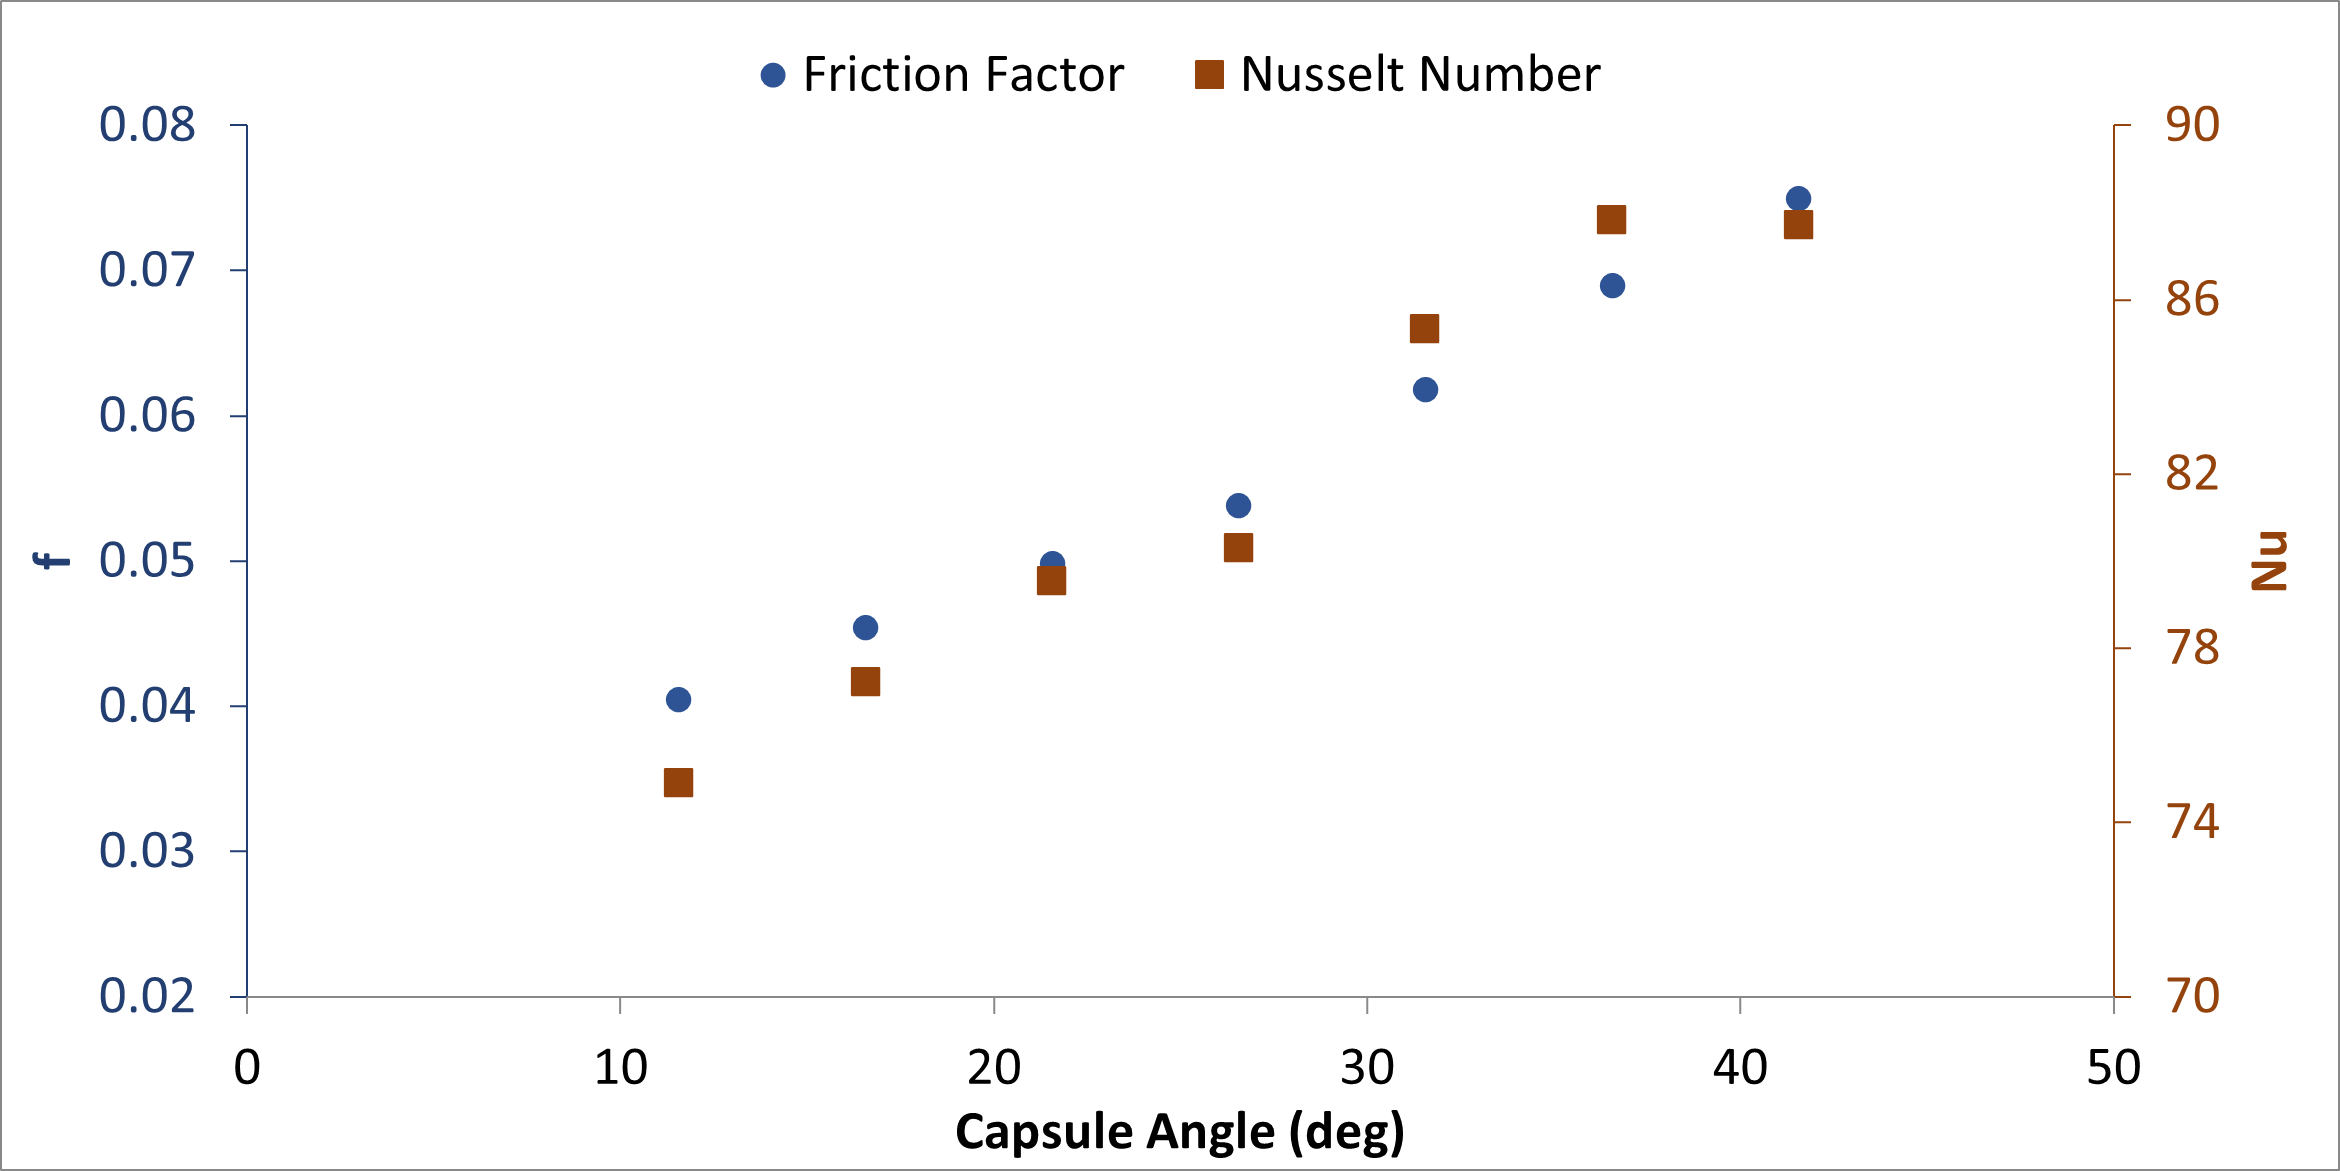
\includegraphics[width=0.7\textwidth, clip, trim=7 2.5 10 5]{media/image114_v1.png}
  \caption{Friction factor and Nusselt number plot vs various capsule angles.}
  \label{figure22}
\end{figure}

\subsection{Capsule height}
\label{sec:disc_capsule_height}

Section~\ref{sec:capsule_height_results} showed that increasing capsule height reduces TKE magnitude, shifts heat transfer from the convex wake to the concave recirculation zones, and slows the mean velocity. These effects produce the quantitative trends in Fig.~\ref{figure23}: both $f$ and Nu rise with capsule height, yet $\Delta p$ simultaneously decreases.

This apparently contradictory behavior---$f$ rising while $\Delta p$ falls---is explained by the Fanning friction factor definition, $f = \Delta p \, D_e / (2\rho \, l_c \, u^2)$. When the gap between the plates widens, the channel cross-section increases, raising $D_e$ and reducing the mean velocity $u$. The larger cross-section lowers the absolute pressure drop $\Delta p$, yet $f$ can still rise because $D_e$ appears in the numerator and $u^2$ in the denominator: both changes push $f$ upward and can outweigh the reduction in $\Delta p$. In physical terms, the friction factor measures the pressure loss relative to the flow's kinetic energy ($\tfrac{1}{2}\rho u^2$); when the flow slows down, even a reduced $\Delta p$ represents a proportionally larger fraction of that kinetic energy, resulting in a higher $f$. The same reasoning applies to the dimple height results discussed in Section~\ref{sec:disc_dimple_height}.

For applications constrained by energy consumption, lower capsule heights (0.09--0.13) are preferable due to their low frictional resistance. Higher capsule heights (0.2--0.22) deliver maximum heat transfer performance for thermally demanding applications. Intermediate capsule heights (0.16--0.18) offer a balanced tradeoff.

\begin{figure}[H]
  \centering
  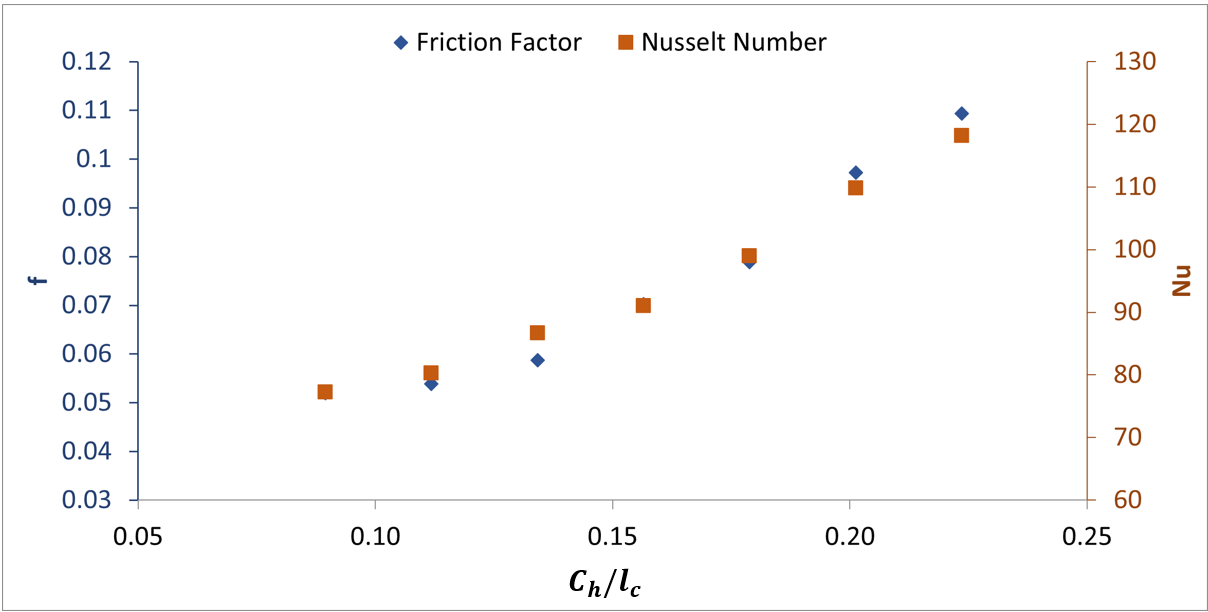
\includegraphics[width=0.7\textwidth, clip, trim=7 5 6 5]{media/image115_v3.png}
  \caption{Friction factor and Nusselt number plot vs various capsule heights/unit cell length.}
  \label{figure23}
\end{figure}

\subsection{Dimple height}
\label{sec:disc_dimple_height}

The flow-field evolution with dimple height (Section~\ref{sec:dimple_height_results}) mirrors the capsule-height trends qualitatively: taller features dampen TKE, enlarge the concave recirculation zone, and shift the primary heat-transfer site away from the convex wake. Quantitatively (Fig.~\ref{figure24}), both $f$ and Nu increase with dimple height, while $\Delta p$ decreases for the same reasons discussed in Section~\ref{sec:disc_capsule_height}.

It is also worth noting that for dimple heights between 0.09 and 0.16, the wake region behind the convex dimple appears more streamlined, extending to the outlet. At $D_h/l_d = 0.18$ the wake experiences significant disruption, causing a noticeable fluctuation in performance (Fig.~\ref{figure24}).

For applications where pumping power must be conserved, lower dimple heights (0.09--0.11) are preferred. Higher dimple heights (0.2--0.22) yield maximum heat transfer performance for thermally demanding systems. Intermediate dimple heights (0.13--0.18) provide a balanced compromise.

\begin{figure}[H]
  \centering
  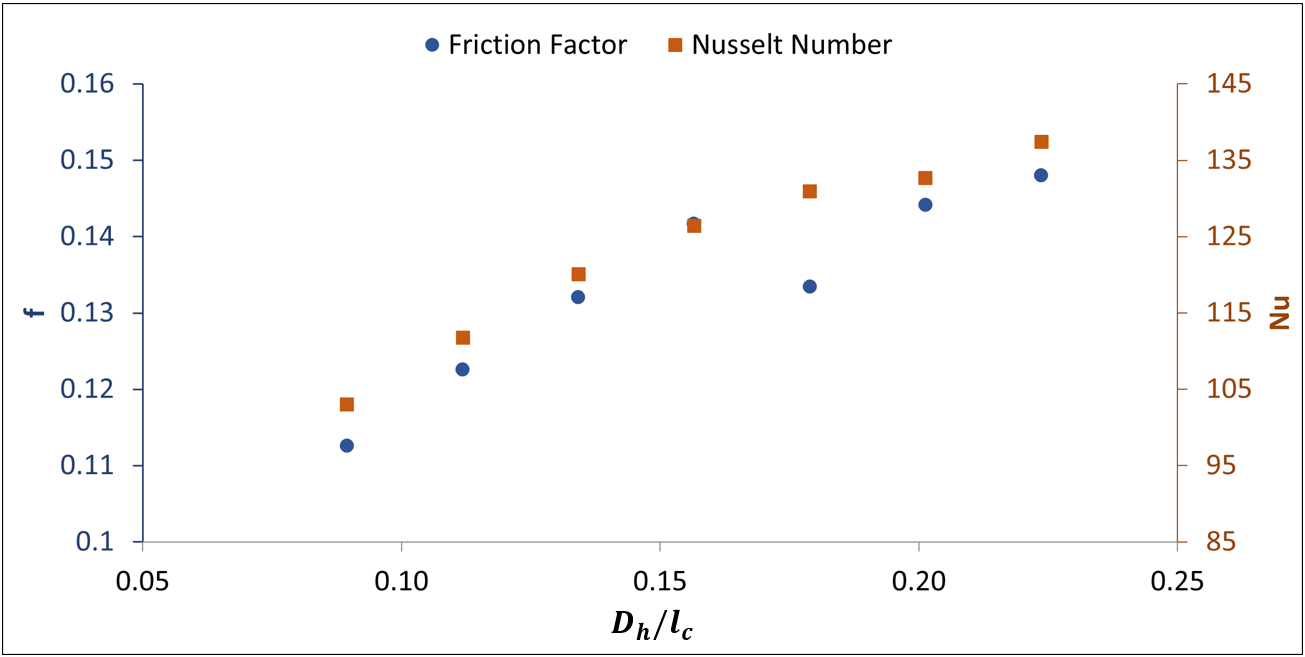
\includegraphics[width=0.7\textwidth, clip, trim={7 5 5 5}]{media/image116_v2.png}
  \caption{Friction factor and Nusselt number plot vs various dimple heights/unit cell length.}
  \label{figure24}
\end{figure}

\subsection{Dimple spacing}
\label{sec:disc_dimple_spacing}

Unlike the three height-based parameters, dimple spacing operates through wake interaction rather than feature size (Section~\ref{sec:dimple_spacing_results}). As the spacing widens, the wake regions behind adjacent dimples become increasingly isolated, reducing turbulence and lowering both $f$ and Nu (Fig.~\ref{figure25}). A distinguishing feature of dimple spacing is that $\Delta p$ remains essentially constant because the dimple height---the primary flow obstruction---is unchanged; only $f$ varies because $D_e$ and $u$ change with the unit-cell length.

Applications requiring high heat transfer efficiency and mechanical stability benefit from closer dimple spacing, while those requiring lower friction factors and clearance from obstruction may prefer wider spacing. Lower friction factors from optimised spacing can reduce pumping energy, leading to significant cost savings in large-scale operations.

\begin{figure}[H]
  \centering
  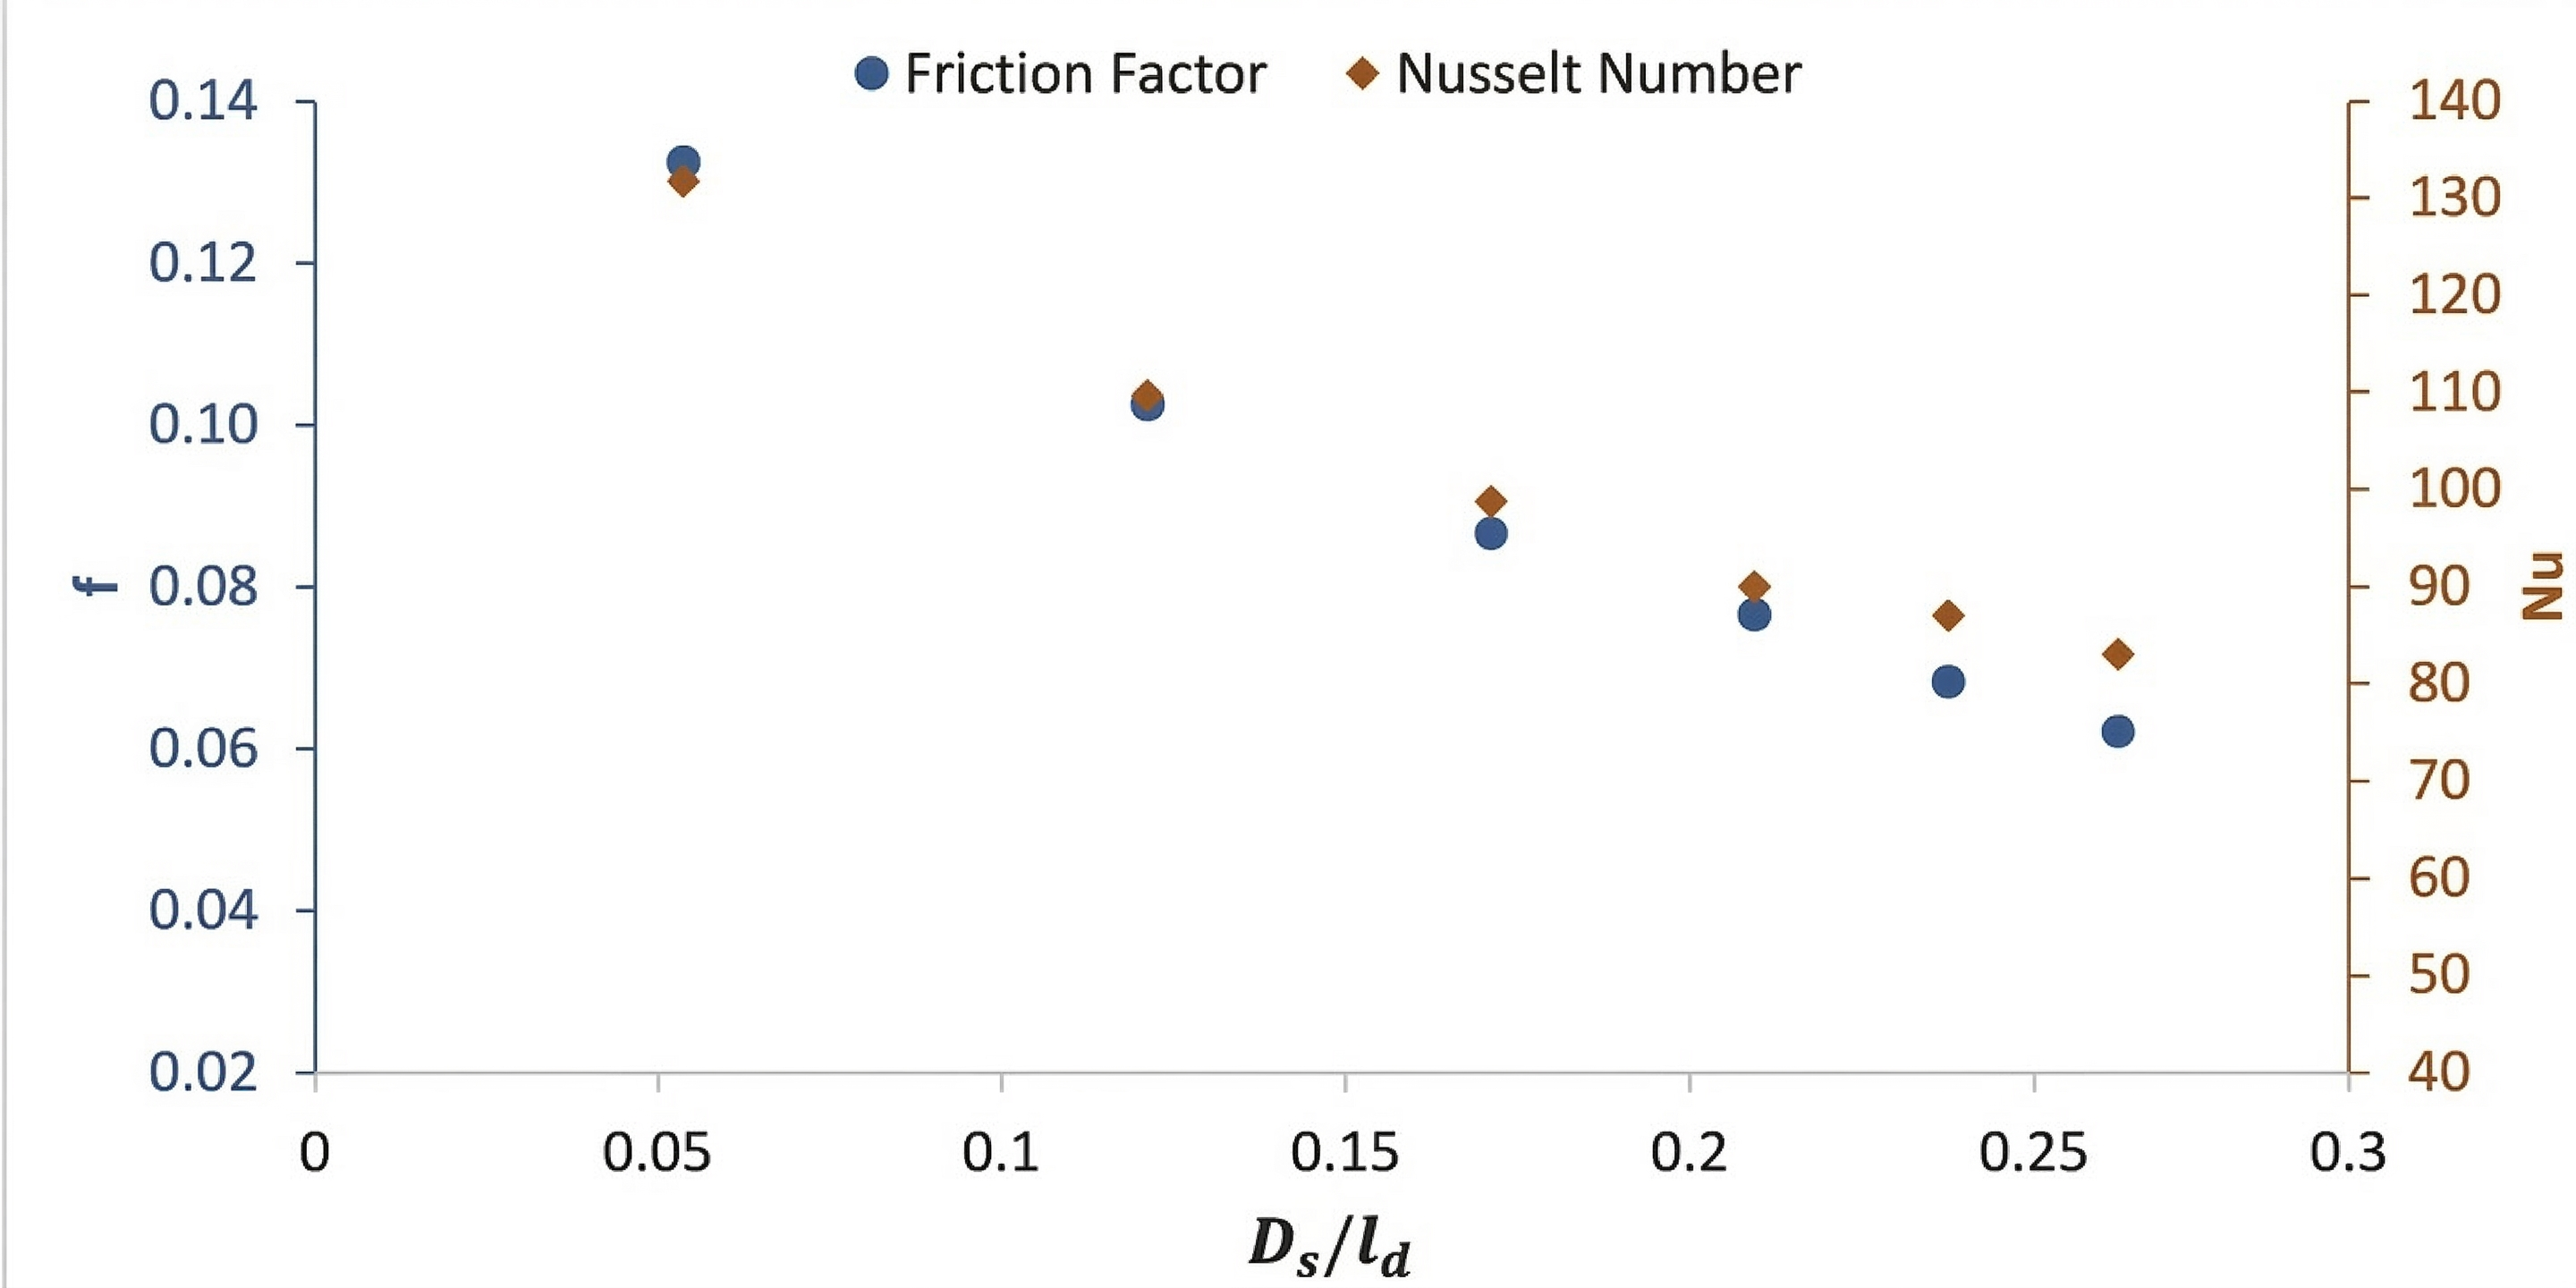
\includegraphics[width=0.7\textwidth, clip, trim={10 5 10 7}]{media/image117_v2.png}
  \caption{Friction factor and Nusselt number plot vs various dimple spacings/unit cell length.}
  \label{figure25}
\end{figure}

\subsection{Cross-parameter thermo-geometric comparison}
\label{sec:tgg_comparison}

Sections~\ref{sec:disc_capsule_angle}--\ref{sec:disc_dimple_spacing} analyzed each geometric parameter in isolation. To compare all four parameters---and both embossing families---on a common scale, the Thermal Performance Factor (Eq.~\eqref{eq:tpf}) is plotted against the Relative Embossing Depth (Eq.~\eqref{eq:red}) for every investigated case in Fig.~\ref{figure_tpf_red}.

\begin{figure}[H]
  \centering
  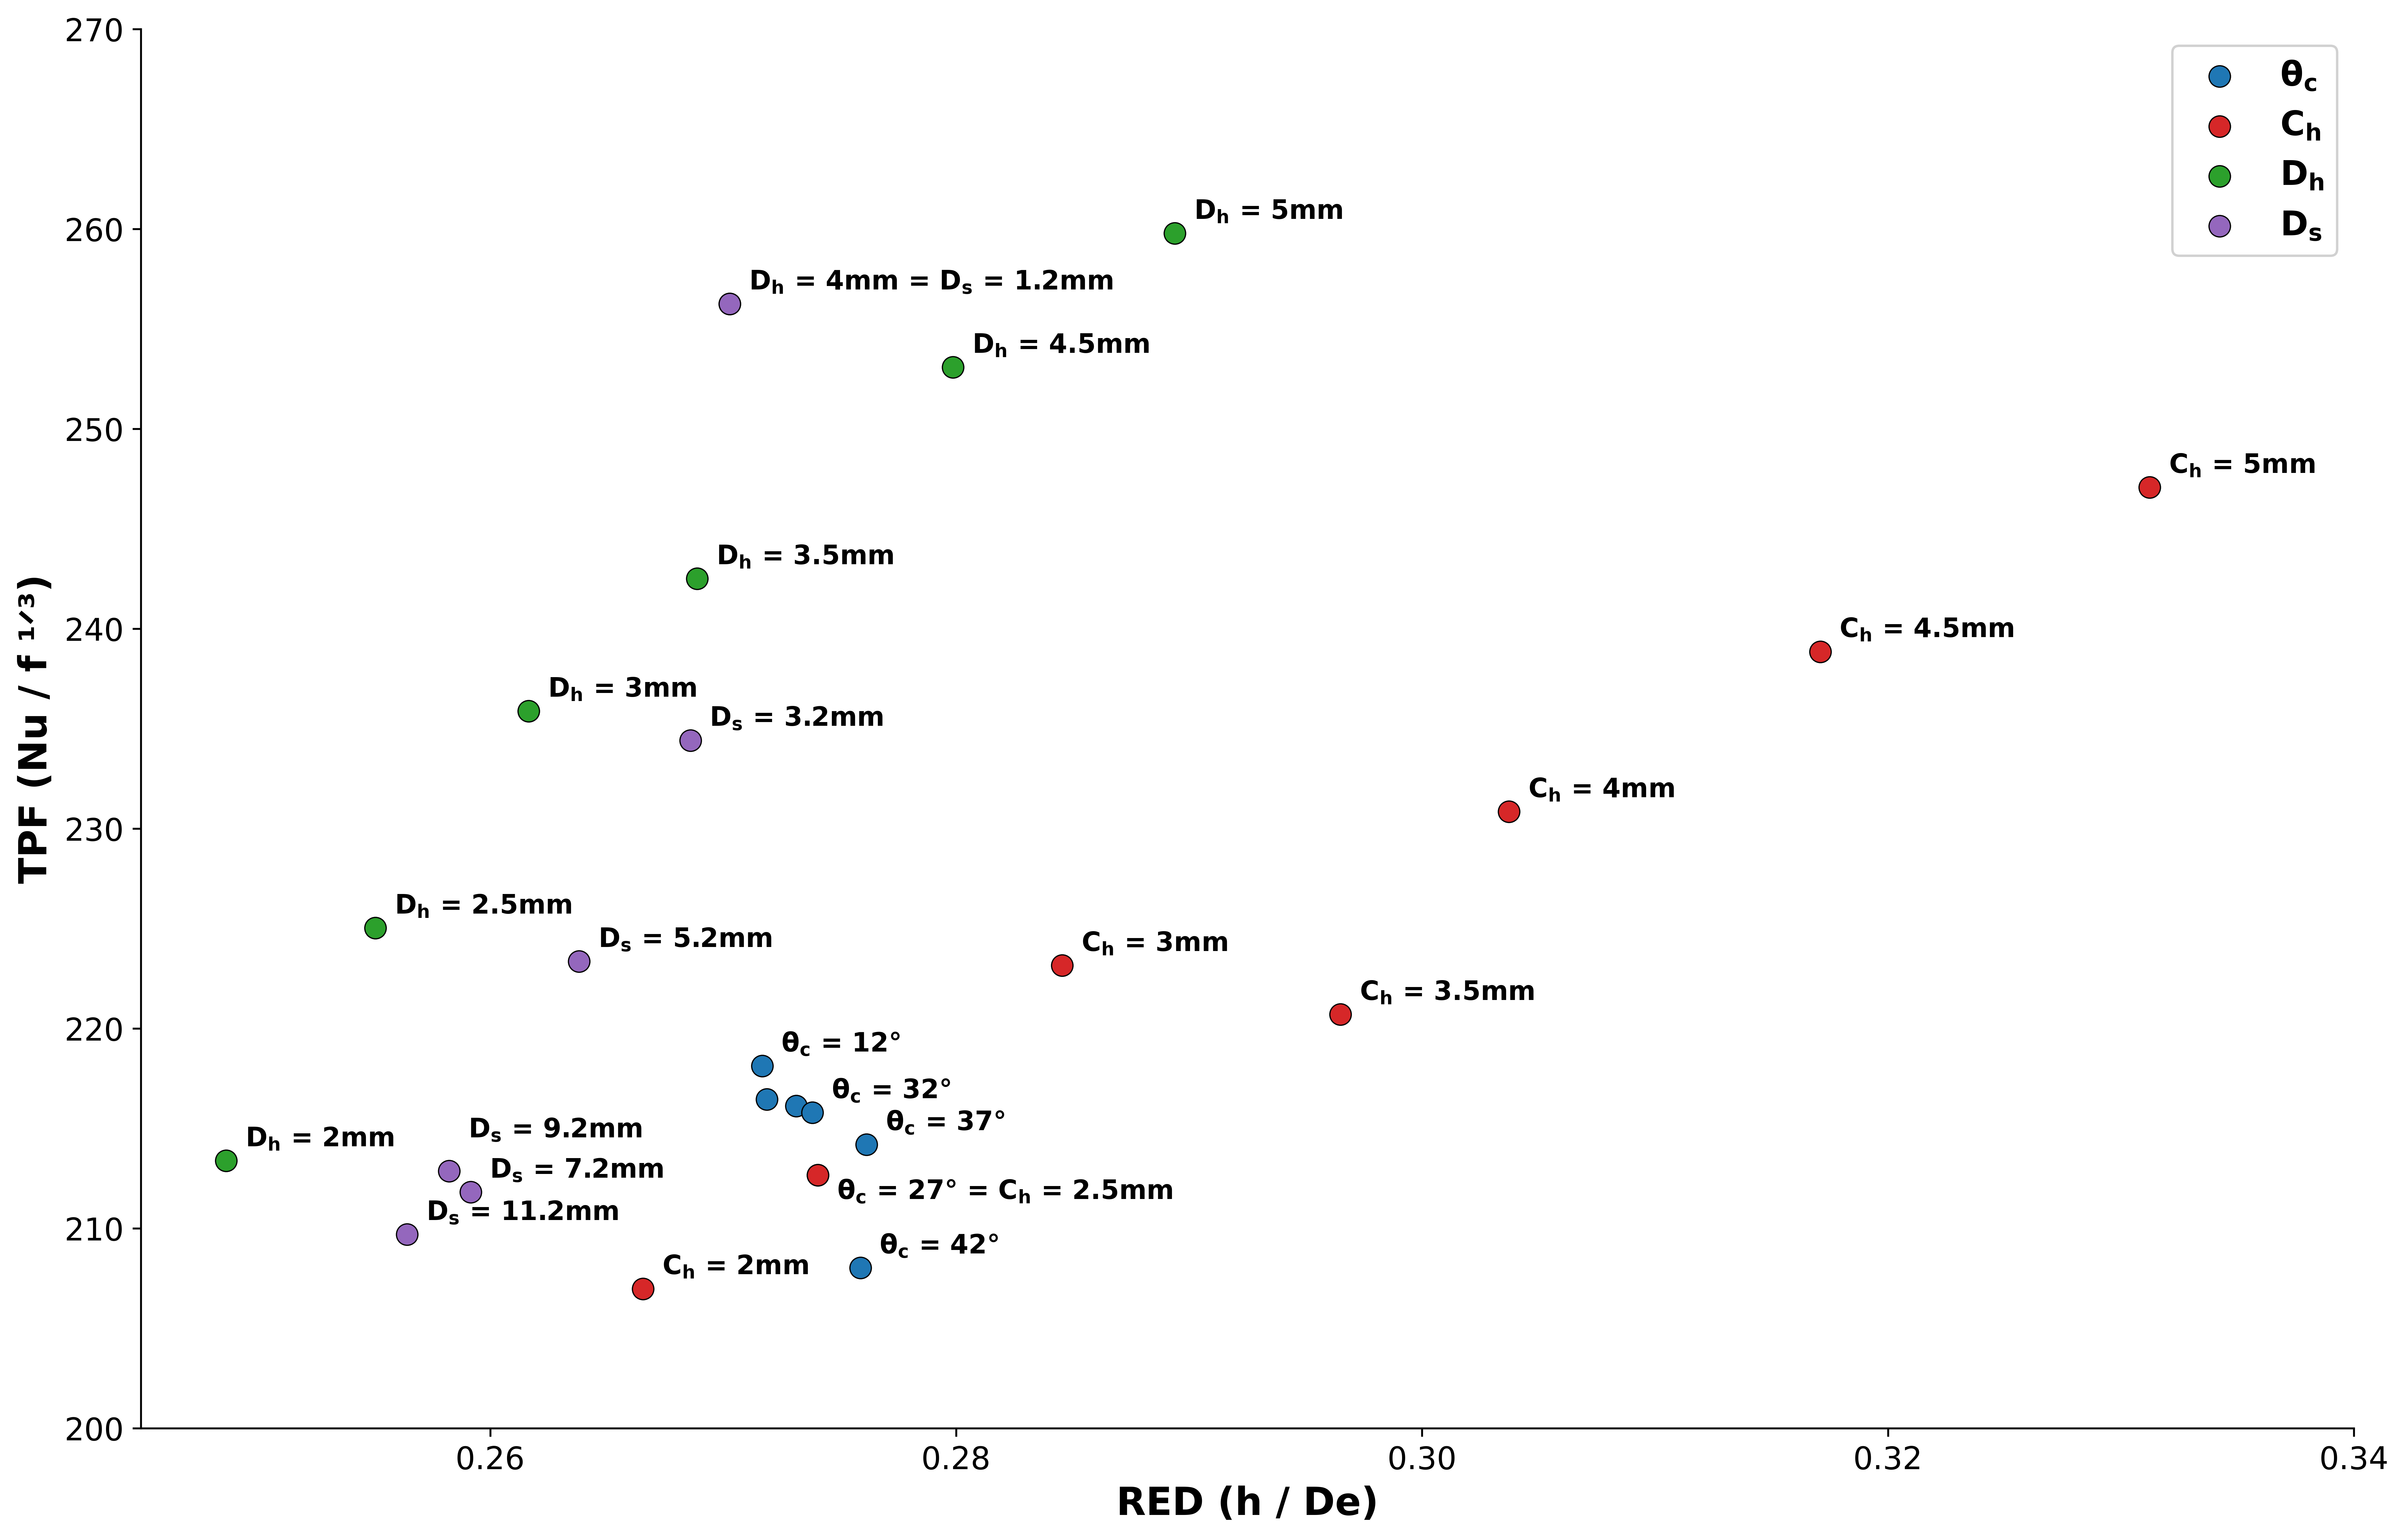
\includegraphics[width=0.7\textwidth]{media/TPF_Vs_RED.png}
  \caption{Thermal Performance Factor (Nu/$f^{1/3}$) versus Relative Embossing Depth (RED\,=\,$h/D_e$) for all 27 parametric cases. Markers distinguish the four parameter families: capsule angle ($\theta_c$), capsule height ($C_h$), dimple height ($D_h$), and dimple spacing ($D_s$).}
  \label{figure_tpf_red}
\end{figure}

Several cross-family observations emerge from the TPF comparison:

\paragraph{Mechanistic differences.}
Within the capsule family, both $\theta_c$ and $C_h$ diminish the wake zone behind the convex capsules---higher angles by redirecting the flow more aggressively, taller capsules by enlarging the cross-sectional area---so that the dominant heat-transfer site shifts from the convex-capsule wake zone at low parameter values to recirculation within the concave capsule cavities at high values. Between families, capsule height and dimple height produce qualitatively similar thermo-hydraulic outcomes (higher Nu at higher $f$) but through different primary mechanisms: physical flow obstruction for capsules versus flow redirection for dimples (see Sections~\ref{sec:disc_capsule_height} and~\ref{sec:disc_dimple_height}). Dimple spacing operates by a distinct mechanism entirely---wake interaction rather than feature size---and is the only parameter for which the overall pressure drop remains essentially unchanged.

\paragraph{Interpretation of TPF vs RED trends.}
The gradient of each family's trend line in Fig.~\ref{figure_tpf_red} quantifies the thermo-hydraulic return per unit change in relative embossing depth and reveals which geometric lever is most efficient. Dimple spacing exhibits the steepest positive gradient ($\approx$\,2950\,TPF\,/\,RED), meaning that even a small reduction in spacing---and hence a modest increase in RED---produces a large TPF gain through intensified wake merging. Dimple height ranks second ($\approx$\,1140\,TPF\,/\,RED), roughly twice as steep as capsule height ($\approx$\,600\,TPF\,/\,RED). Comparing these two families, $D_h$ cases achieve the highest absolute TPF values overall, confirming that flow redirection---which enhances turbulence and mixing within the concave cavities---is a more effective augmentation mechanism than physical flow obstruction at comparable embossing depths. Capsule angle is the only family with a negative gradient ($\approx$\,$-$1460\,TPF\,/\,RED): although higher angles raise Nu, the accompanying rise in $f$ is disproportionately large, so increasing the angle raises RED marginally while degrading TPF through separation losses. These gradients reinforce the design recommendation that, for a given manufacturing investment in embossing depth, dimple spacing and dimple height adjustments offer the greatest thermo-hydraulic payoff, whereas capsule angle changes should be avoided as a primary benchmarking route.

\begin{figure}[H]
  \centering
  \includegraphics[width=0.8\textwidth]{media/TPF_Design_Ranking.png}
  \caption{TPF design ranking of all 27 parametric cases.}
  \label{design_ranking}
\end{figure}

\paragraph{Design ranking.}
Fig.~\ref{design_ranking} ranks all 27 cases by TPF along the $y$-axis. The five highest-ranked cases are all from the dimple family: $D_h$\,=\,5.0\,mm leads, followed by $D_h$\,=\,4.0\,mm (tied with $D_s$\,=\,1.2\,mm because it is the same geometry), and $D_h$\,=\,4.5\,mm. The highest-ranked capsule case ($C_h$\,=\,5.0\,mm) appears only in sixth place, confirming that dimple-type embossing delivers superior thermo-hydraulic performance in the tested configurations (noting that TPF is evaluated at each case's own converged Reynolds number; see Section~\ref{sec:performance_criteria}). Within each family the trend is consistent: for the three height-based parameters ($C_h$, $D_h$, $D_s$ at fixed height), taller features rank higher because the Nu gain outpaces the friction penalty scaled by $f^{1/3}$. By contrast, all capsule-angle cases cluster in the lower half of the ranking ($\theta_c$\,=\,12\degree\ is the highest at 15th overall, $\theta_c$\,=\,42\degree\ is 25th), indicating that increasing the capsule angle is the least efficient route to improving thermal performance. Dimple spacing follows a clear monotonic trend: the closest spacing ($D_s$\,=\,1.2\,mm, tied 2nd) ranks far above the widest ($D_s$\,=\,11.2\,mm, 24th), reinforcing the finding that wake merging from closely packed dimples substantially enhances heat transfer without a proportionate friction penalty. For thermally demanding applications (e.g.\ high-density data-center cooling for AI infrastructure), the results recommend tall dimples ($D_h$\,$\geq$\,4.0\,mm) or closely spaced dimples ($D_s$\,$\leq$\,3.2\,mm). Where pumping power must be conserved and only moderate heat transfer is required, capsule designs at low angles ($\theta_c$\,$\leq$\,17\degree) or low heights ($C_h$\,$\leq$\,3.0\,mm) offer an acceptable compromise, albeit at considerably lower absolute TPF.

\subsection{Limitations of this study}
\label{sec:limitations}

Exploring the intricacies of heat exchanger designs through numerical investigations can be incredibly enlightening, yet it is important to remember these methods are not without their flaws. Recognizing these limitations helps us better understand the results and spot areas that need more research and real-world testing.

For instance, our study assumes that the working fluid does not compress, making the calculations simpler. However, this assumption does not hold up for all real-world scenarios, especially when dealing with gases or other compressible fluids. Additionally, our simulations only consider single-phase flow, meaning they do not take into account the complexities that come with multiphase flows like liquid-gas. These interactions can drastically change heat transfer and pressure drops. Moreover, the boundary conditions we apply in simulations tend to be idealized. They do not always reflect the varied and sometimes chaotic conditions found in real-life operations, such as changing inlet temperatures or pressures. We also assume that the physical properties of the working fluid, like density, viscosity, and thermal conductivity, remain constant. In reality, these properties can change significantly with temperature and pressure, which affects both flow and heat transfer.

While our numerical results offer valuable insights, it is crucial to validate them with experimental data to ensure they are accurate and reliable. Unfortunately, finding experimental data for specific configurations and conditions can be a challenge, which can slow down the validation process.


\section{Conclusion}
\label{sec:conclusion}

This study presented a unified, unit-cell CFD benchmarking of two non-chevron plate heat exchanger families---capsule-type (CPHE) and dimple-type (DPHE)---covering 27 parametric cases across four geometric variables: capsule angle ($\theta_c$), capsule height ($C_h$), dimple height ($D_h$), and dimple spacing ($D_s$). A periodic unit-cell reduction strategy with a consistent hydraulic-diameter definition was adopted to ensure an apples-to-apples comparison of every configuration.

For CPHE, increasing capsule angle intensifies flow disturbance, raising both the friction factor and Nu, but the friction penalty grows disproportionately, yielding diminishing thermo-hydraulic returns at higher angles. Increasing capsule height raises the friction factor through greater flow obstruction; however, the larger cross-section reduces the mean velocity, and the resulting pressure drop is expected to decrease even as $f$ rises---a consequence of the Fanning friction factor definition in which $D_e$ and $u^2$ appear in the numerator and denominator, respectively. In both $\theta_c$ and $C_h$ cases, the dominant heat-transfer mechanism shifts from the convex-capsule wake zone at low parameter values to recirculation within the concave capsule cavities at high values.

For DPHE, increasing dimple height produces a qualitatively similar outcome to capsule height---higher $f$, higher Nu, and a lower expected pressure drop---but through flow redirection rather than physical obstruction. Dimple spacing governs wake interaction: closer spacing merges the wakes behind adjacent dimples, elevating turbulence, $f$, and Nu, while the overall pressure drop remains effectively unchanged because the primary flow obstruction (dimple height) is held constant.

Two cross-family metrics were introduced to enable a direct comparison of all 27 cases. A Relative Embossing Depth (RED\,=\,$h/D_e$) provides a unified dimensionless geometric axis that captures how every modification---whether an angle, a height, or a spacing---ultimately alters the ratio of embossing protrusion to effective channel size. A Thermal Performance Factor (TPF\,=\,Nu/$f^{1/3}$) serves as a relative thermo-hydraulic ranking index evaluated at each case's own converged operating state, requiring no auxiliary geometric normalization.

The TPF-vs-RED comparison shows that dimple-type plates consistently outperform capsule-type plates. The five highest-ranked cases are all from the dimple family: $D_h$\,=\,5.0\,mm leads, followed by $D_h$\,=\,4.0\,mm (tied with $D_s$\,=\,1.2\,mm), and $D_h$\,=\,4.5\,mm. The best capsule case ($C_h$\,=\,5.0\,mm) ranks only sixth. All capsule-angle cases occupy the lower half of the ranking (15th--25th of 27), confirming that varying the capsule angle is the least efficient route to improving thermal performance. For thermally demanding applications---such as high-density data-center liquid cooling for AI infrastructure---the results recommend tall dimples ($D_h$\,$\geq$\,4.0\,mm) or closely spaced dimples ($D_s$\,$\leq$\,3.2\,mm). Where pumping power must be conserved and only moderate heat transfer is required, capsule designs at low angles ($\theta_c$\,$\leq$\,17\degree) or low heights ($C_h$\,$\leq$\,3.0\,mm) offer an acceptable compromise at considerably lower absolute TPF.

The findings should be interpreted in light of the modeling assumptions (incompressible, single-phase flow; idealized boundary conditions; constant fluid properties), and experimental validation remains an important next step. Future work should also examine plate structural integrity (e.g.\ via nonlinear transient FEM) and extend the analysis across Reynolds numbers and working fluids to broaden design applicability.

\section*{Declaration of competing interests}

The authors declare that they have no known competing financial interests or personal relationships that could have appeared to influence the work reported in this paper.

\section*{Credit authorship contribution statement}

\textbf{Cheuk Sing Cheung:} Conceptualization, Methodology, Software, Formal analysis, Investigation, Data curation, Writing, Visualization. \textbf{Christos Skarakis:} Conceptualization, Methodology, Software, Formal analysis, Investigation, Data curation, Writing, Visualization. \textbf{Lance Smith:} Resources, Supervision. \textbf{Sara Vahaji:} Conceptualization, Methodology, Supervision, Writing -- review \& editing, Project administration.

\section*{Declaration of generative AI and AI-assisted technologies in the manuscript preparation process}

No generative AI or AI-assisted technologies were used in the preparation of this manuscript.

\section*{Acknowledgements}

Inkorr Pty Ltd. provided resources for this research.

\section*{Funding}

This research did not receive any specific grant from funding agencies in the public, commercial, or not-for-profit sectors.


\nocite{*}
\bibliography{references}

\end{document}
